% ============================================================================
% VaN3Twin en Docker sobre macOS (Apple Silicon) — Guía detallada
% Compilar con: pdflatex VaN3Twin_Docker_macOS.tex  (2 pasadas)
% ============================================================================
\documentclass[11pt,a4paper]{article}

\usepackage[utf8]{inputenc}
\usepackage[T1]{fontenc}
\usepackage{lmodern}
\usepackage[margin=2.2cm]{geometry}
\usepackage{xcolor}
\usepackage{amssymb}
\usepackage{graphicx}
\usepackage{booktabs}
\usepackage{array}
\usepackage{listings}
\usepackage{tikz}
\usetikzlibrary{shapes.geometric, arrows.meta, positioning, fit}
\usepackage[most]{tcolorbox}
\usepackage[hidelinks]{hyperref}
\usepackage{fancyhdr}

% --- Nombres en español (sin babel) ---------------------------------------
\renewcommand{\contentsname}{\'Indice de contenidos}
\renewcommand{\figurename}{Figura}
\renewcommand{\tablename}{Tabla}
\renewcommand{\abstractname}{Resumen}
\renewcommand{\appendixname}{Anexo}

% --- Colores ----------------------------------------------------------------
\definecolor{codebg}{RGB}{245,246,248}
\definecolor{codeframe}{RGB}{200,204,210}
\definecolor{kwcolor}{RGB}{160,32,120}
\definecolor{strcolor}{RGB}{34,120,50}
\definecolor{comcolor}{RGB}{120,128,140}
\definecolor{boxinfo}{RGB}{225,238,252}
\definecolor{boxwarn}{RGB}{253,240,220}
\definecolor{boximp}{RGB}{232,246,232}
\definecolor{drivex}{RGB}{20,60,110}

% --- Listings ---------------------------------------------------------------
\lstset{
  basicstyle=\ttfamily\footnotesize,
  backgroundcolor=\color{codebg},
  frame=single, rulecolor=\color{codeframe}, framesep=4pt,
  breaklines=true, breakatwhitespace=true,
  postbreak=\mbox{\textcolor{comcolor}{$\hookrightarrow$}\space},
  showstringspaces=false,
  keywordstyle=\color{kwcolor}\bfseries,
  stringstyle=\color{strcolor},
  commentstyle=\color{comcolor}\itshape,
  tabsize=2, columns=fullflexible, keepspaces=true,
  extendedchars=true, inputencoding=utf8,
  literate={á}{{\'a}}1 {é}{{\'e}}1 {í}{{\'i}}1 {ó}{{\'o}}1 {ú}{{\'u}}1
           {ñ}{{\~n}}1 {Á}{{\'A}}1 {É}{{\'E}}1 {Í}{{\'I}}1 {Ó}{{\'O}}1
           {Ú}{{\'U}}1 {Ñ}{{\~N}}1 {—}{{---}}1 {–}{{--}}1
           {¿}{{?`}}1 {¡}{{!`}}1 {ü}{{\"u}}1
}
\lstdefinelanguage{Dockerfile}{
  morekeywords={FROM,RUN,CMD,LABEL,MAINTAINER,EXPOSE,ENV,ADD,COPY,
    ENTRYPOINT,VOLUME,USER,WORKDIR,ARG,ONBUILD,STOPSIGNAL,HEALTHCHECK,SHELL},
  sensitive=true, morecomment=[l]{\#}, morestring=[b]", morestring=[b]'
}
\lstdefinelanguage{yaml}{
  keywords={true,false,null,yes,no},
  sensitive=false, morecomment=[l]{\#}, morestring=[b]', morestring=[b]"
}

% --- Cajas ------------------------------------------------------------------
\newtcolorbox{implicacion}{colback=boximp, colframe=green!45!black,
  title=Implicaci\'on, fonttitle=\bfseries, left=2mm, right=2mm, top=1mm, bottom=1mm}
\newtcolorbox{nota}{colback=boxinfo, colframe=blue!55!black,
  title=Nota, fonttitle=\bfseries, left=2mm, right=2mm, top=1mm, bottom=1mm}
\newtcolorbox{advertencia}{colback=boxwarn, colframe=orange!75!black,
  title=Advertencia, fonttitle=\bfseries, left=2mm, right=2mm, top=1mm, bottom=1mm}

% --- Estilos TikZ para diagramas de flujo -----------------------------------
\tikzset{
  inicio/.style={ellipse, draw=drivex, fill=drivex!12, thick,
    minimum height=8mm, align=center, font=\small},
  proceso/.style={rectangle, rounded corners=2pt, draw=drivex, fill=white,
    thick, minimum height=8mm, minimum width=30mm, align=center, font=\small},
  procesoc/.style={proceso, fill=drivex!8},
  decision/.style={diamond, aspect=2.2, draw=orange!80!black,
    fill=orange!10, thick, align=center, font=\small, inner sep=1pt},
  datos/.style={trapezium, trapezium left angle=70, trapezium right angle=110,
    draw=green!45!black, fill=green!8, thick, align=center, font=\small},
  flecha/.style={-{Stealth[length=2.5mm]}, thick, color=black!70},
  etiq/.style={font=\scriptsize\itshape, color=black!60}
}

\pagestyle{fancy}
\fancyhf{}
\fancyhead[L]{\small VaN3Twin en Docker --- macOS Apple Silicon}
\fancyhead[R]{\small\thepage}
\renewcommand{\headrulewidth}{0.4pt}

\title{\textbf{Instalaci\'on de VaN3Twin en Docker}\\[2mm]
\large Gu\'ia detallada paso a paso para macOS Tahoe sobre Apple Silicon\\[1mm]
\normalsize Repositorio: \url{https://github.com/DriveX-devs/VaN3Twin}}
\author{Pablo Barbecho \\ \small Universidad de Cuenca}
\date{Agosto 2026}

\begin{document}
\maketitle
\thispagestyle{empty}

\begin{abstract}
\noindent
VaN3Twin (evoluci\'on del framework \emph{ms-van3t} del Politecnico di Torino /
DriveX) es un conjunto de m\'odulos para ns-3 que permite construir y simular
aplicaciones VANET/V2X conformes con ETSI, acoplando el simulador de red ns-3
con el simulador de movilidad SUMO mediante TraCI. El proyecto \textbf{no}
ofrece soporte oficial de Docker: su instalaci\'on nativa asume Ubuntu
(20.04/22.04/24.04) y un script interactivo (\texttt{sandbox\_builder.sh}).
Este documento analiza el software y su proceso de instalaci\'on, y presenta
una contenedorizaci\'on completa y reproducible para Docker Desktop en macOS
Tahoe con Apple Silicon (arm64): un \texttt{Dockerfile} explicado capa por
capa, un \texttt{docker-compose.yml} comentado directiva por directiva, el
soporte de interfaz gr\'afica (\texttt{sumo-gui}) v\'ia VNC integrado
(Xvfb + x11vnc, con XQuartz como alternativa), y las
implicaciones t\'ecnicas de cada decisi\'on.
\end{abstract}

\tableofcontents
\newpage

% ============================================================================
\section{An\'alisis del software VaN3Twin}
% ============================================================================

\subsection{Qu\'e es y de d\'onde viene}

VaN3Twin es el nuevo nombre del framework \emph{ms-van3t}; integra todas sus
funcionalidades y a\~nade otras nuevas (p.\,ej.\ la integraci\'on con el
ray-tracer NVIDIA Sionna). Es un conjunto de m\'odulos para
\textbf{ns-3} (versi\'on \texttt{ns-3-dev} del fork 5G-LENA de CTTC, con
soporte del m\'odulo NR-V2X) que permite simular comunicaciones vehiculares
V2X con pila ETSI ITS-G5 completa (mensajes CAM, DENM, CPM, VAM, IVIM,
en versiones v1 y v2 con ASN.1 real), pudiendo conmutar f\'acilmente la
tecnolog\'ia de acceso: IEEE 802.11p, LTE, C-V2X Modo 4 y NR-V2X.
La movilidad de los veh\'iculos proviene de \textbf{SUMO} (versiones probadas:
1.6.0 a 1.18.0), acoplado en tiempo de simulaci\'on mediante \textbf{TraCI}.
Licencia GPL-2.0.

\subsection{Estructura del repositorio}

Los componentes principales dentro de \texttt{src/} son:

\begin{center}
\small
\begin{tabular}{@{}p{0.26\textwidth}p{0.66\textwidth}@{}}
\toprule
\textbf{M\'odulo} & \textbf{Funci\'on} \\
\midrule
\texttt{automotive} & Pila ETSI ITS-G5 (CAM/DENM/CPM/VAM, ASN.1, DCC,
facilities), aplicaciones de ejemplo y mapas SUMO. Requiere OpenSSL y
\textbf{OpenCV} (\texttt{find\_package(OpenCV REQUIRED)}). \\
\texttt{traci}, \texttt{traci-applications} & L\'ogica de acoplamiento
ns-3 $\leftrightarrow$ SUMO (cliente TraCI). \\
\texttt{cv2x} & Modelo C-V2X (LTE-V2X) en modo de transmisi\'on 4. \\
\texttt{nr} & M\'odulo 5G-LENA con NR-V2X (se descarga aparte, rama
\texttt{nr-v2x-dev}). \\
\texttt{gps-tc} & Reproducci\'on de trazas GPS reales como movilidad. \\
\texttt{carla} & Cliente gRPC hacia CARLA/OpenCDA (percepci\'on y
movilidad). Requiere \textbf{gRPC con ficheros CMake}
(\texttt{find\_package(gRPC CONFIG REQUIRED)}). \\
\texttt{sionna} & Integraci\'on con el ray-tracer NVIDIA Sionna
(canal radio realista). \\
\texttt{vehicle-visualizer} & Visualizador web (Node.js) de los
veh\'iculos: servidor HTTP + socket UDP interno 48110. \\
\bottomrule
\end{tabular}
\end{center}

\begin{figure}[h!]
\centering
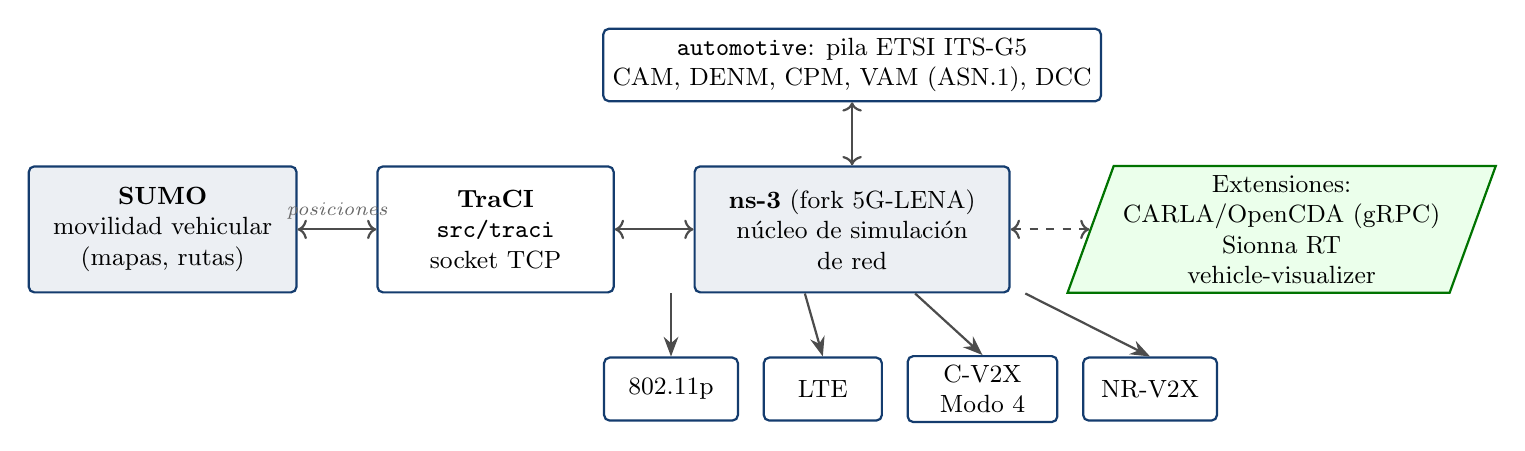
\begin{tikzpicture}[node distance=6mm and 8mm]
  % SUMO
  \node[procesoc, minimum width=34mm, minimum height=16mm] (sumo)
    {\textbf{SUMO}\\movilidad vehicular\\(mapas, rutas)};
  % TraCI
  \node[proceso, right=10mm of sumo, minimum height=16mm] (traci)
    {\textbf{TraCI}\\\texttt{src/traci}\\socket TCP};
  % ns-3 core
  \node[procesoc, right=10mm of traci, minimum width=40mm, minimum height=16mm] (ns3)
    {\textbf{ns-3} (fork 5G-LENA)\\n\'ucleo de simulaci\'on\\de red};
  % pila ETSI encima
  \node[proceso, above=8mm of ns3, minimum width=40mm] (etsi)
    {\textbf{\texttt{automotive}}: pila ETSI ITS-G5\\CAM, DENM, CPM, VAM (ASN.1), DCC};
  % tecnologías debajo
  \node[proceso, below=8mm of ns3, minimum width=17mm, xshift=-23mm] (wifi) {802.11p};
  \node[proceso, right=3mm of wifi, minimum width=15mm] (lte) {LTE};
  \node[proceso, right=3mm of lte, minimum width=19mm] (cv2x) {C-V2X\\Modo 4};
  \node[proceso, right=3mm of cv2x, minimum width=17mm] (nr) {NR-V2X};
  % extensiones a la derecha
  \node[datos, right=10mm of ns3, minimum height=8mm] (ext)
    {Extensiones:\\CARLA/OpenCDA (gRPC)\\Sionna RT\\vehicle-visualizer};
  \draw[flecha, <->] (sumo) -- node[etiq, above]{posiciones} (traci);
  \draw[flecha, <->] (traci) -- (ns3);
  \draw[flecha, <->] (etsi) -- (ns3);
  \draw[flecha] (ns3.south) ++(-23mm,0) -- (wifi.north);
  \draw[flecha] (ns3.south) ++(-6mm,0) -- (lte.north);
  \draw[flecha] (ns3.south) ++(8mm,0) -- (cv2x.north);
  \draw[flecha] (ns3.south) ++(22mm,0) -- (nr.north);
  \draw[flecha, <->, dashed] (ns3) -- (ext);
\end{tikzpicture}
\caption{Arquitectura funcional de VaN3Twin: SUMO aporta la movilidad, TraCI
la sincroniza con ns-3, y la pila ETSI ITS-G5 se ejecuta sobre la tecnolog\'ia
de acceso elegida.}
\label{fig:arquitectura}
\end{figure}

\subsection{C\'omo se instala nativamente (y por qu\'e importa para Docker)}

El README oficial define este procedimiento sobre Ubuntu:
instalar SUMO; clonar el repo; ejecutar \texttt{./sandbox\_builder.sh}
(con \texttt{install-dependencies} la primera vez); y finalmente
\texttt{./ns3 configure} + \texttt{./ns3 build} dentro de
\texttt{ns-3-dev/}. El script \texttt{sandbox\_builder.sh} tiene varias
particularidades que \textbf{condicionan el dise\~no del Dockerfile}:

\begin{enumerate}
  \item \textbf{Rechaza ejecutarse como root} (\texttt{if [ "\$EUID" -eq 0 ]
  ... exit 1}). En Docker el usuario por defecto es root, as\'i que hay que
  crear un usuario sin privilegios.
  \item \textbf{Es interactivo}: contiene \texttt{read -p "Press ENTER to
  continue..."}. En una build no interactiva hay que alimentarle la entrada
  (\texttt{echo "" | ./sandbox\_builder.sh}).
  \item \textbf{Detecta la versi\'on de Ubuntu} con \texttt{lsb\_release} y
  solo acepta 20.04, 22.04 o 24.04. La imagen base debe ser una de ellas y
  tener instalado \texttt{lsb-release}.
  \item Con \texttt{install-dependencies} compila \textbf{gRPC v1.60.0 y
  OpenCV desde c\'odigo fuente} (horas de CPU). En Docker conviene separar
  esto en capas cacheables y sustituir OpenCV por el paquete apt.
  \item Clona el ns-3 de CTTC (etiqueta \texttt{ns-3-dev-v2x-v0.2}) y el
  m\'odulo \texttt{nr} (rama \texttt{nr-v2x-dev}), copia los m\'odulos de
  VaN3Twin dentro de \texttt{ns-3-dev/src/}, aplica parches (modelos de
  propagaci\'on extendidos, SignalInfo, ficheros Sionna) y
  \textbf{se auto-elimina} (\texttt{rm \$0}) al terminar.
  \item En Ubuntu 22.04+ el \texttt{configure} exige
  \texttt{--disable-werror}; en 24.04 adem\'as
  \texttt{CXXFLAGS="-include cstdint"}.
\end{enumerate}

\begin{figure}[h!]
\centering
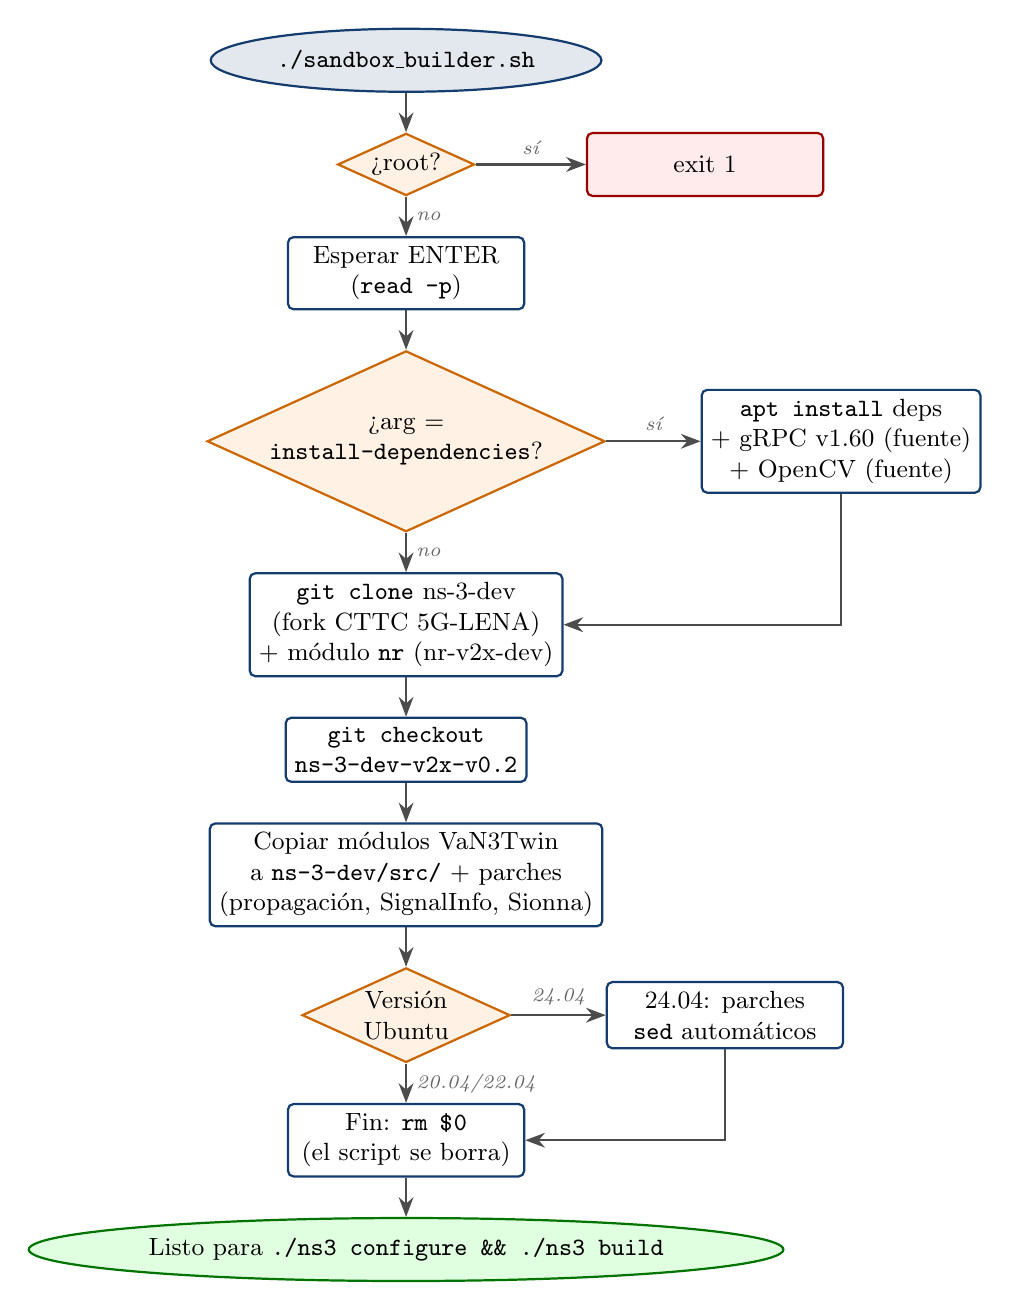
\begin{tikzpicture}[node distance=5mm]
  \node[inicio] (a) {\texttt{./sandbox\_builder.sh}};
  \node[decision, below=of a] (root) {\textquestiondown root?};
  \node[proceso, right=14mm of root, fill=red!8, draw=red!60!black] (exit1) {exit 1};
  \node[proceso, below=of root] (enter) {Esperar ENTER\\(\texttt{read -p})};
  \node[decision, below=of enter] (dep) {\textquestiondown arg =\\\texttt{install-dependencies}?};
  \node[proceso, right=12mm of dep] (apt) {\texttt{apt install} deps\\+ gRPC v1.60 (fuente)\\+ OpenCV (fuente)};
  \node[proceso, below=of dep] (clone) {\texttt{git clone} ns-3-dev\\(fork CTTC 5G-LENA)\\+ m\'odulo \texttt{nr} (nr-v2x-dev)};
  \node[proceso, below=of clone] (tag) {\texttt{git checkout}\\\texttt{ns-3-dev-v2x-v0.2}};
  \node[proceso, below=of tag] (copy) {Copiar m\'odulos VaN3Twin\\a \texttt{ns-3-dev/src/} + parches\\(propagaci\'on, SignalInfo, Sionna)};
  \node[decision, below=of copy] (ubu) {Versi\'on\\Ubuntu};
  \node[proceso, right=12mm of ubu] (u24) {24.04: parches\\\texttt{sed} autom\'aticos};
  \node[proceso, below=of ubu] (fin) {Fin: \texttt{rm \$0}\\(el script se borra)};
  \node[inicio, below=of fin, fill=green!12, draw=green!45!black] (listo)
    {Listo para \texttt{./ns3 configure \&\& ./ns3 build}};
  \draw[flecha] (a) -- (root);
  \draw[flecha] (root) -- node[etiq, above]{s\'i} (exit1);
  \draw[flecha] (root) -- node[etiq, right]{no} (enter);
  \draw[flecha] (enter) -- (dep);
  \draw[flecha] (dep) -- node[etiq, above]{s\'i} (apt);
  \draw[flecha] (dep) -- node[etiq, right]{no} (clone);
  \draw[flecha] (apt) |- (clone);
  \draw[flecha] (clone) -- (tag);
  \draw[flecha] (tag) -- (copy);
  \draw[flecha] (copy) -- (ubu);
  \draw[flecha] (ubu) -- node[etiq, above]{24.04} (u24);
  \draw[flecha] (ubu) -- node[etiq, right]{20.04/22.04} (fin);
  \draw[flecha] (u24) |- (fin);
  \draw[flecha] (fin) -- (listo);
\end{tikzpicture}
\caption{Flujo interno de \texttt{sandbox\_builder.sh}. Las decisiones
marcadas condicionan el dise\~no del Dockerfile (usuario no root, entrada
no interactiva, \texttt{lsb-release}, dependencias pre-instaladas).}
\label{fig:sandbox}
\end{figure}

\clearpage

% ============================================================================
\section{Estrategia de contenedorizaci\'on para macOS Apple Silicon}
% ============================================================================

\subsection{C\'omo funciona Docker en un Mac}

En macOS, Docker Desktop no ejecuta contenedores ``directamente'': crea una
\textbf{m\'aquina virtual Linux ligera} (Virtualization.framework) y todos los
contenedores viven dentro de esa VM. Esto tiene tres implicaciones directas
para VaN3Twin:

\begin{implicacion}
\begin{itemize}
  \item \textbf{Recursos}: la RAM/CPU/disco que ve el contenedor son los
  asignados a la VM en \emph{Docker Desktop $\to$ Settings $\to$ Resources},
  no los del Mac. Compilar ns-3 con 8 hilos puede requerir 10--16\,GB de RAM
  de la VM.
  \item \textbf{E/S de ficheros}: los \emph{bind mounts} (carpetas del Mac
  montadas en el contenedor) pasan por VirtioFS y son m\'as lentos que el
  disco interno de la VM. Aun as\'i, este proyecto monta el \'arbol completo
  de VaN3Twin como bind mount (\texttt{./VaN3Twin}) para tenerlo visible en
  el Finder y editable con VS Code desde el Mac; el coste se nota sobre todo
  en builds completos de ns-3 (ediciones y simulaciones apenas lo acusan).
  \item \textbf{Red}: no hay acceso directo a las interfaces f\'isicas del
  Mac (ni \texttt{macvlan}); el modo emulaci\'on de VaN3Twin
  (\texttt{v2x-emulator} sobre una NIC real) no es viable en este entorno.
\end{itemize}
\end{implicacion}

\subsection{Decisiones de dise\~no y sus implicaciones}

\begin{center}
\small
\begin{tabular}{@{}p{0.30\textwidth}p{0.62\textwidth}@{}}
\toprule
\textbf{Decisi\'on} & \textbf{Justificaci\'on e implicaci\'on} \\
\midrule
Base \texttt{ubuntu:22.04} & Es una de las tres versiones aceptadas por
\texttt{sandbox\_builder.sh}; existe imagen arm64 oficial; evita los parches
extra de 24.04. Obliga a usar \texttt{--disable-werror}. \\
Arquitectura \texttt{linux/arm64} & Nativa en Apple Silicon: sin emulaci\'on
Rosetta, compilaci\'on 2--5$\times$ m\'as r\'apida. Todo se construye desde
fuente o desde paquetes multi-arch, as\'i que no hay dependencias x86\_64. \\
SUMO 1.12.0 desde repos Ubuntu (no PPA) & Los PPA de Launchpad
(\texttt{ppa:sumo/stable}) normalmente no publican binarios arm64
$\Rightarrow$ fallar\'ia en Apple Silicon. Adem\'as 1.12.0 est\'a dentro del
rango probado (1.6--1.18) y el README advierte contra versiones m\'as nuevas
de TraCI. \\
gRPC v1.60.0 desde fuente & Obligatorio: \texttt{src/carla} usa
\texttt{find\_package(gRPC CONFIG REQUIRED)} y el paquete apt de 22.04 no
trae los ficheros CMake de gRPC. A\~nade $\sim$30--45 min de build (una sola
vez, queda cacheado en una capa). \\
OpenCV desde apt (\texttt{libopencv-dev}) & \texttt{src/automotive} solo
necesita \texttt{find\_package(OpenCV)}; OpenCV 4.5.4 de Ubuntu lo satisface.
Evita $\sim$40 min de compilaci\'on y $\sim$2\,GB de imagen frente al
procedimiento del script oficial. \\
Sin \texttt{libc6-dev-i386} & Ese paquete solo existe en amd64; en arm64
romper\'ia el \texttt{apt install}. No es necesario para compilar VaN3Twin. \\
Usuario \texttt{vanet} no root & \texttt{sandbox\_builder.sh} aborta si
detecta root. Adem\'as es buena pr\'actica de seguridad; se le da
\texttt{sudo} sin contrase\~na para comodidad en desarrollo. \\
Build completo \textbf{dentro} de la imagen & La imagen queda ``lista para
simular'' (\texttt{docker compose up} y ejecutar). Contrapartida: imagen
grande ($\sim$10--15\,GB) y build inicial largo (1--3 h). \\
Volumen nombrado sobre el \'arbol ns-3 & Persiste ediciones y recompilaciones
entre recreaciones del contenedor con E/S r\'apida (disco de la VM). \\
GUI v\'ia VNC (Xvfb + x11vnc en el contenedor) & \texttt{sumo-gui} necesita
un servidor X con GLX; el X virtual interno lo aporta por software
(llvmpipe) sin depender del Mac. Visor: \emph{Compartir pantalla} de macOS
(\texttt{vnc://127.0.0.1:5901}). XQuartz queda como alternativa opcional. \\
\bottomrule
\end{tabular}
\end{center}

\begin{advertencia}
\textbf{Limitaciones en Mac/Docker} que conviene conocer desde el principio:
\begin{itemize}
  \item \textbf{Extensi\'on CARLA/OpenCDA}: CARLA 0.9.12 se distribuye solo
  como binario \texttt{x86\_64} y recomienda GPU NVIDIA $\geq$8\,GB. No es
  ejecutable de forma \'util en Apple Silicon (ni con Rosetta). El m\'odulo
  \texttt{carla} de ns-3 \emph{se compila} igualmente (por eso se instala
  gRPC), pero el simulador CARLA deber\'ia correr en una m\'aquina Linux
  x86\_64 remota.
  \item \textbf{Sionna}: la GPU NVIDIA \emph{no} es obligatoria --- el ray
  tracer funciona en CPU (backend LLVM de Dr.Jit). La secci\'on~\ref{sec:sionna}
  detalla la soluci\'on recomendada sin GPU: servidor Sionna \textbf{nativo en
  el Mac} conectado al contenedor por UDP. Para estudios grandes sigue siendo
  preferible una m\'aquina remota con GPU.
  \item \textbf{Modo emulaci\'on} (\texttt{v2x-emulator}): requiere una NIC
  real; la VM de Docker Desktop no la expone.
\end{itemize}
Nada de esto afecta al uso principal: \textbf{simulaciones V2X completas
(802.11p, LTE, C-V2X, NR-V2X) con SUMO, incluida la GUI}.
\end{advertencia}

\clearpage

% ============================================================================
\section{Prerrequisitos en el Mac (macOS Tahoe)}
% ============================================================================

\subsection{Software necesario}

\begin{lstlisting}[language=bash, caption={Instalaci\'on de prerrequisitos con Homebrew}]
# 1. Docker Desktop (runtime de contenedores con VM Linux integrada)
brew install --cask docker

# 2. Para la GUI de SUMO NO se necesita nada más: va por VNC y el visor
#    ("Compartir pantalla") viene integrado en macOS.
#    XQuartz solo si prefieres la alternativa X11 (ver 3.3):
# brew install --cask xquartz

# 3. Verificaciones
docker --version          # Docker version 27.x o superior
docker compose version    # Docker Compose version v2.x
uname -m                  # arm64  (Apple Silicon)
\end{lstlisting}

\subsection{Configurar recursos de Docker Desktop}

En \emph{Docker Desktop $\to$ Settings $\to$ Resources}:

\begin{center}
\small
\begin{tabular}{@{}lll@{}}
\toprule
\textbf{Recurso} & \textbf{M\'inimo} & \textbf{Recomendado} \\
\midrule
CPUs      & 4        & 6--8 \\
Memoria   & 8\,GB    & 12--16\,GB \\
Swap      & 1\,GB    & 2\,GB \\
Disco virtual & 40\,GB & 60--80\,GB \\
\bottomrule
\end{tabular}
\end{center}

\begin{implicacion}
La compilaci\'on de ns-3 lanza un proceso \texttt{g++} por n\'ucleo y algunos
ficheros ASN.1 del m\'odulo \texttt{automotive} consumen 1--2\,GB de RAM cada
uno al compilarse con \texttt{-O2}. Si la VM tiene poca memoria, el kernel de
la VM matar\'a procesos (\texttt{g++: internal compiler error: Killed}) y la
build fallar\'a. Regla pr\'actica: $\text{RAM de la VM} \geq 1.5 \times
\text{CPUs asignadas}$ en GB.
\end{implicacion}

\subsection{(Opcional) Configurar XQuartz --- solo para la alternativa X11}
\label{sec:xquartzconf}

\textbf{Con la GUI por VNC (m\'etodo por defecto, \S\ref{sec:vnc}) esta
secci\'on no es necesaria}: no hay nada que instalar ni configurar en el Mac.
Sigue estos pasos \'unicamente si decides usar la variante XQuartz (X11 en
red), que requiere adem\'as activar las l\'ineas comentadas
\texttt{DISPLAY}/\texttt{LIBGL\_ALWAYS\_INDIRECT} del compose.

\begin{enumerate}
  \item Abrir XQuartz, men\'u \emph{XQuartz $\to$ Settings $\to$ Security} y
  marcar \textbf{``Allow connections from network clients''}.
  \item Habilitar el \textbf{GLX indirecto} (XQuartz lo trae desactivado por
  defecto; sin \'el, \texttt{sumo-gui} abre la ventana pero el canvas OpenGL
  falla con \texttt{X Error: GLXBadContext} y el mapa no se dibuja):
\begin{lstlisting}[language=bash]
defaults write org.xquartz.X11 enable_iglx -bool true
\end{lstlisting}
  \item Cerrar XQuartz por completo y volver a abrirlo (o reiniciar el Mac)
  para aplicar ambos cambios.
  \item Antes de cada sesi\'on con GUI, autorizar al cliente local:
\end{enumerate}

\begin{lstlisting}[language=bash]
/opt/X11/bin/xhost + 127.0.0.1
# la VM de Docker Desktop llega al host vía NAT y aparece como 127.0.0.1
\end{lstlisting}

\begin{advertencia}
\texttt{xhost + 127.0.0.1} permite que \emph{cualquier} proceso local se
conecte a tu pantalla X11 mientras XQuartz est\'e abierto. Es aceptable en un
equipo personal; rev\'ocalo al terminar con \texttt{xhost - 127.0.0.1} o
cerrando XQuartz.
\end{advertencia}

\subsection{Flujo general de la instalaci\'on}

\begin{figure}[h!]
\centering
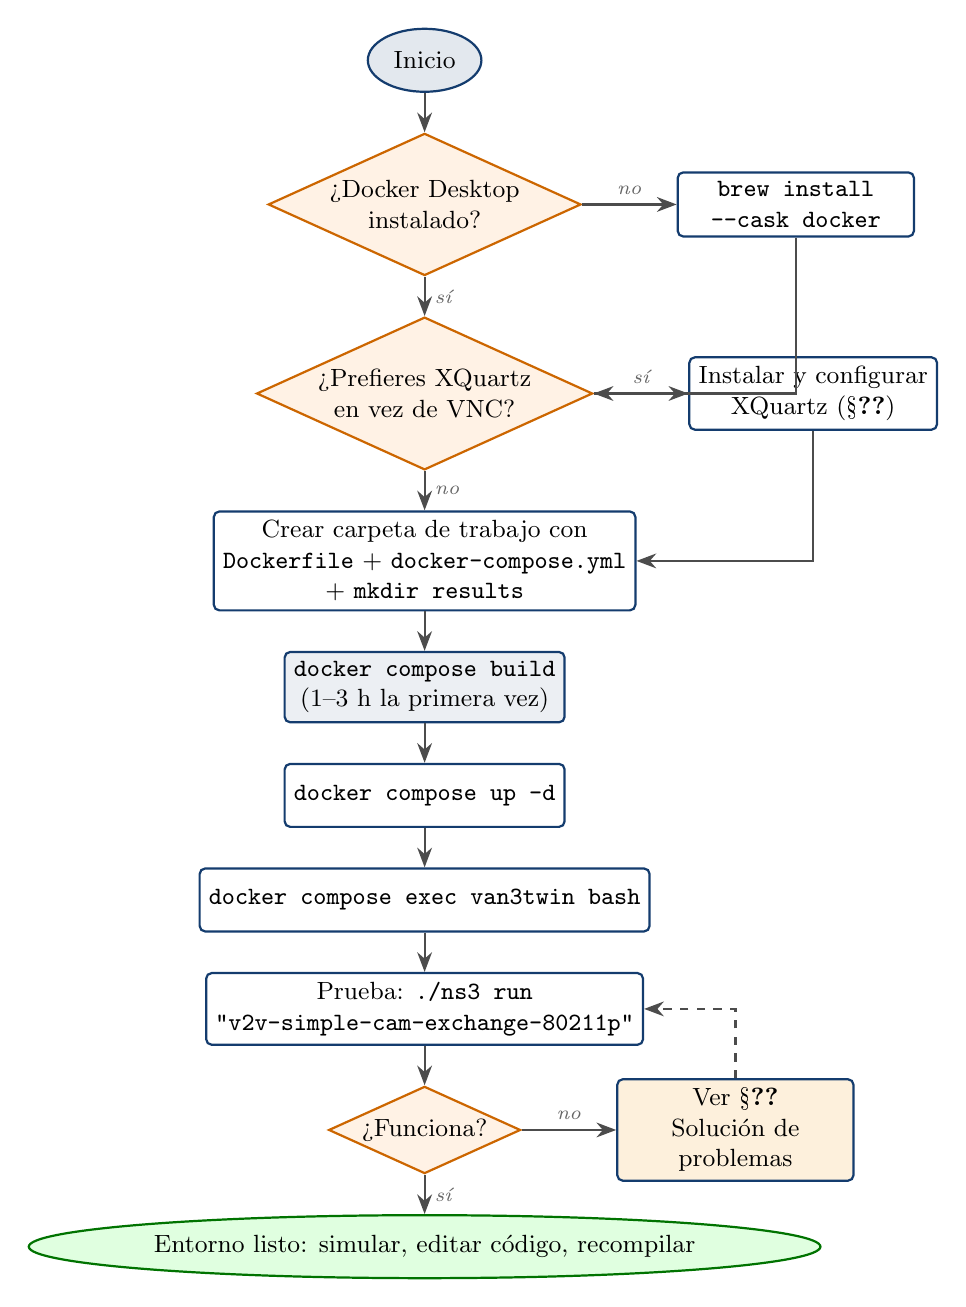
\begin{tikzpicture}[node distance=5mm]
  \node[inicio] (ini) {Inicio};
  \node[decision, below=of ini] (dd) {\textquestiondown Docker Desktop\\instalado?};
  \node[proceso, right=12mm of dd] (idd) {\texttt{brew install}\\\texttt{--cask docker}};
  \node[decision, below=of dd] (xq) {\textquestiondown Prefieres XQuartz\\en vez de VNC?};
  \node[proceso, right=12mm of xq] (ixq) {Instalar y configurar\\XQuartz (\S\ref{sec:xquartzconf})};
  \node[proceso, below=of xq] (files) {Crear carpeta de trabajo con\\\texttt{Dockerfile} + \texttt{docker-compose.yml}\\+ \texttt{mkdir results}};
  \node[proceso, below=of files, fill=drivex!8] (build) {\texttt{docker compose build}\\(1--3 h la primera vez)};
  \node[proceso, below=of build] (up) {\texttt{docker compose up -d}};
  \node[proceso, below=of up] (exec) {\texttt{docker compose exec van3twin bash}};
  \node[proceso, below=of exec] (test) {Prueba: \texttt{./ns3 run}\\\texttt{"v2v-simple-cam-exchange-80211p"}};
  \node[decision, below=of test] (ok) {\textquestiondown Funciona?};
  \node[proceso, right=12mm of ok, fill=boxwarn] (tr) {Ver \S\ref{sec:trouble}\\Soluci\'on de\\problemas};
  \node[inicio, below=of ok, fill=green!12, draw=green!45!black] (fin)
    {Entorno listo: simular, editar c\'odigo, recompilar};
  \draw[flecha] (ini) -- (dd);
  \draw[flecha] (dd) -- node[etiq, above]{no} (idd);
  \draw[flecha] (idd) |- (xq);
  \draw[flecha] (dd) -- node[etiq, right]{s\'i} (xq);
  \draw[flecha] (xq) -- node[etiq, above]{s\'i} (ixq);
  \draw[flecha] (ixq) |- (files);
  \draw[flecha] (xq) -- node[etiq, right]{no} (files);
  \draw[flecha] (files) -- (build);
  \draw[flecha] (build) -- (up);
  \draw[flecha] (up) -- (exec);
  \draw[flecha] (exec) -- (test);
  \draw[flecha] (test) -- (ok);
  \draw[flecha] (ok) -- node[etiq, above]{no} (tr);
  \draw[flecha] (ok) -- node[etiq, right]{s\'i} (fin);
  \draw[flecha, dashed] (tr) |- (test);
\end{tikzpicture}
\caption{Flujo general de la instalaci\'on de VaN3Twin en Docker sobre macOS.}
\label{fig:flujogeneral}
\end{figure}

\clearpage

% ============================================================================
\section{El Dockerfile, capa por capa}
% ============================================================================

El c\'odigo de la imagen vive \'unicamente en el fichero \texttt{Dockerfile}
de la carpeta de trabajo (fuente de verdad; no se duplica aqu\'i para evitar
desincronizaci\'on). Esta secci\'on explica cada capa y sus implicaciones. La figura~\ref{fig:capas} resume el
pipeline.

\begin{figure}[h!]
\centering
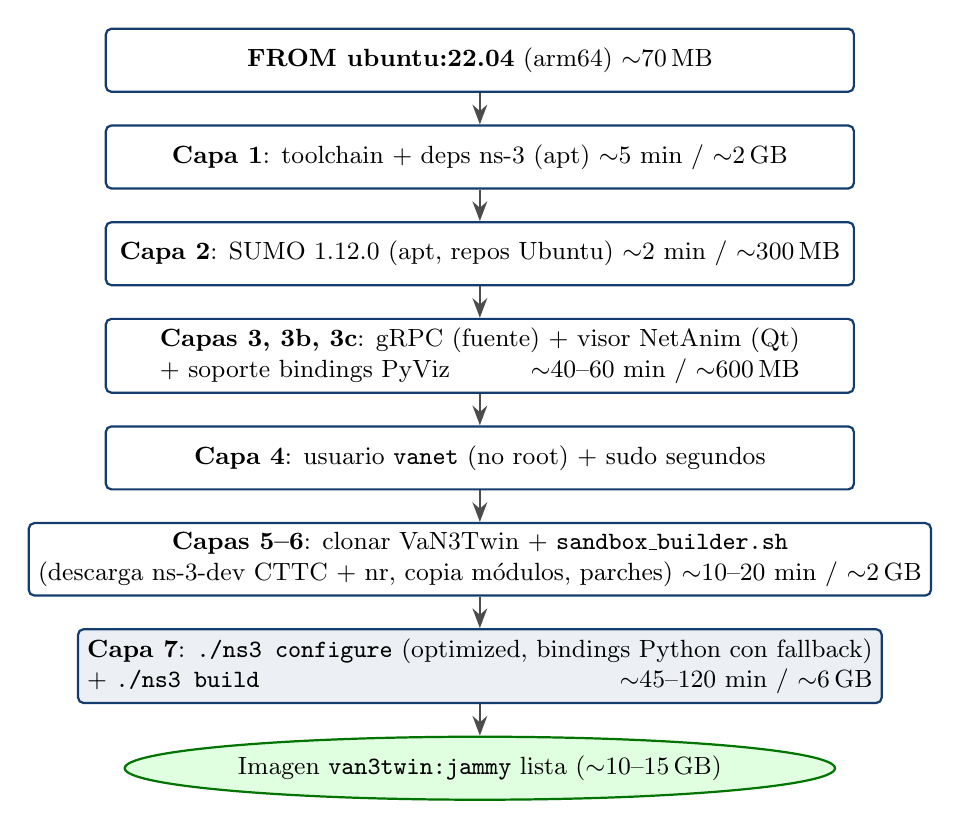
\begin{tikzpicture}[node distance=4mm]
  \node[proceso, minimum width=95mm] (base) {\textbf{FROM ubuntu:22.04} (arm64) \hfill $\sim$70\,MB};
  \node[proceso, minimum width=95mm, below=of base] (l1)
    {\textbf{Capa 1}: toolchain + deps ns-3 (apt) \hfill $\sim$5 min / $\sim$2\,GB};
  \node[proceso, minimum width=95mm, below=of l1] (l2)
    {\textbf{Capa 2}: SUMO 1.12.0 (apt, repos Ubuntu) \hfill $\sim$2 min / $\sim$300\,MB};
  \node[proceso, minimum width=95mm, below=of l2] (l3)
    {\textbf{Capas 3, 3b, 3c}: gRPC (fuente) + visor NetAnim (Qt)\\+ soporte bindings PyViz \hfill $\sim$40--60 min / $\sim$600\,MB};
  \node[proceso, minimum width=95mm, below=of l3] (l4)
    {\textbf{Capa 4}: usuario \texttt{vanet} (no root) + sudo \hfill segundos};
  \node[proceso, minimum width=95mm, below=of l4] (l5)
    {\textbf{Capas 5--6}: clonar VaN3Twin + \texttt{sandbox\_builder.sh}\\
     (descarga ns-3-dev CTTC + nr, copia m\'odulos, parches) \hfill $\sim$10--20 min / $\sim$2\,GB};
  \node[proceso, minimum width=95mm, below=of l5, fill=drivex!8] (l6)
    {\textbf{Capa 7}: \texttt{./ns3 configure} (optimized, bindings Python con fallback)\\
     + \texttt{./ns3 build} \hfill $\sim$45--120 min / $\sim$6\,GB};
  \node[inicio, below=of l6, fill=green!12, draw=green!45!black] (img)
    {Imagen \texttt{van3twin:jammy} lista ($\sim$10--15\,GB)};
  \draw[flecha] (base) -- (l1);
  \draw[flecha] (l1) -- (l2);
  \draw[flecha] (l2) -- (l3);
  \draw[flecha] (l3) -- (l4);
  \draw[flecha] (l4) -- (l5);
  \draw[flecha] (l5) -- (l6);
  \draw[flecha] (l6) -- (img);
\end{tikzpicture}
\caption{Pipeline de capas del Dockerfile con tiempos orientativos en un
M2/M3 con 6 CPUs y 12\,GB asignados a Docker. Cada capa se cachea: si algo
falla o se cambia, solo se reconstruye desde la capa modificada hacia abajo.}
\label{fig:capas}
\end{figure}

\subsection{Cabecera y argumentos}

\begin{implicacion}
\texttt{DEBIAN\_FRONTEND=noninteractive} evita que paquetes como
\texttt{tzdata} detengan la build pidiendo la zona horaria por teclado
(cl\'asico bloqueo de builds Docker con Ubuntu). Al declararlo como
\texttt{ARG} (y no \texttt{ENV}) solo aplica durante la construcci\'on, no
queda ``pegado'' en los contenedores. \texttt{GRPC\_VERSION} y
\texttt{VAN3TWIN\_REF} permiten fijar versiones reproducibles desde el
\texttt{docker-compose.yml} sin editar el Dockerfile.
\end{implicacion}

\subsection{Capa 1 --- Toolchain y dependencias}

La lista replica la de \texttt{sandbox\_builder.sh install-dependencies} con
cuatro ajustes razonados:

\begin{itemize}
  \item \textbf{Se omite \texttt{libc6-dev-i386}}: no existe para arm64; su
  inclusi\'on romper\'ia la build en Apple Silicon. Solo sirve para compilar
  binarios de 32 bits en x86, algo que VaN3Twin no necesita.
  \item \textbf{Se a\~nade \texttt{libopencv-dev}} en lugar de compilar
  OpenCV desde fuente (ver \S2.2).
  \item \textbf{Se a\~naden \texttt{libgl1-mesa-dri} y \texttt{mesa-utils}}:
  el driver software de Mesa (\texttt{swrast}/\texttt{llvmpipe}) permite que
  \texttt{sumo-gui} renderice OpenGL \emph{dentro} del contenedor con
  \texttt{LIBGL\_ALWAYS\_SOFTWARE=1}, sin depender del GLX de XQuartz. Sin
  este paquete se produce \texttt{libGL error: failed to load driver: swrast}
  y una lluvia de \texttt{GLXBadContext}. \texttt{mesa-utils} aporta
  \texttt{glxinfo}/\texttt{glxgears} para diagnosticar.
  \item \textbf{Se omiten los paquetes de bindings Python de ns-3}
  (\texttt{gir1.2-goocanvas}, \texttt{python3-pygraphviz}, etc.) porque el
  \texttt{configure} usa \texttt{--disable-python}.
\end{itemize}

\begin{implicacion}
\texttt{--no-install-recommends} reduce cientos de MB de paquetes sugeridos.
\texttt{rm -rf /var/lib/apt/lists/*} en el \emph{mismo} \texttt{RUN} borra los
\'indices de apt antes de que la capa se selle: si se hiciera en otro
\texttt{RUN}, el espacio ya estar\'ia consumido en la capa anterior (las capas
son inmutables y aditivas). \texttt{lsb-release} y \texttt{sudo} no son
opcionales: el primero lo exige la detecci\'on de versi\'on de
\texttt{sandbox\_builder.sh}; el segundo da flexibilidad al usuario no root.
\end{implicacion}

\subsection{Capa 2 --- SUMO}

\begin{implicacion}
Ubuntu 22.04 empaqueta SUMO \textbf{1.12.0} para arm64 y amd64, dentro del
rango probado por los autores (1.6.0--1.18.0). El README oficial sugiere el
PPA \texttt{ppa:sumo/stable}, pero (a) los PPA rara vez publican arm64, y
(b) instalar\'ia un SUMO m\'as nuevo cuya API TraCI podr\'ia no ser
compatible (``\emph{Back compatibility is not ensured with new versions of
TraCI}''). \texttt{SUMO\_HOME} es le\'ido por las herramientas de SUMO
(p.\,ej.\ \texttt{randomTrips.py}, \texttt{netconvert}) y por scripts del
framework. El paquete \texttt{sumo} incluye \texttt{sumo-gui}.
\end{implicacion}

\subsection{Capa 3 --- gRPC desde c\'odigo fuente}

\begin{implicacion}
Es la capa ``cara'' que no se puede evitar: \texttt{src/carla/CMakeLists.txt}
ejecuta \texttt{find\_package(gRPC CONFIG REQUIRED)}, que busca los ficheros
\texttt{gRPCConfig.cmake} --- el paquete \texttt{libgrpc++-dev} de Ubuntu
22.04 \textbf{no los incluye}, de ah\'i que el script oficial tambi\'en
compile gRPC v1.60.0 desde fuente. Detalles del comando:
\texttt{--depth 1} y \texttt{--init --depth 1} clonan solo el \'ultimo commit
(ahorra $\sim$1\,GB de descarga); \texttt{-DgRPC\_BUILD\_TESTS=OFF} recorta
mucho tiempo; y el \texttt{rm -rf /opt/grpc} final, al estar en el mismo
\texttt{RUN}, evita que $\sim$6\,GB de fuentes y objetos queden fosilizados
en la capa. \texttt{ldconfig} refresca la cach\'e del enlazador para que
\texttt{/usr/local/lib} sea visible.
\end{implicacion}

\subsection{Capa 4 --- Usuario no root}

\begin{implicacion}
Sin esta capa, \texttt{sandbox\_builder.sh} abortar\'ia con \emph{``Please do
NOT run this script as root''}. A partir del \texttt{USER vanet}, todas las
instrucciones siguientes (y la shell del contenedor en ejecuci\'on) corren
como usuario normal: los ficheros creados en los vol\'umenes tendr\'an un
propietario coherente y se reduce la superficie de ataque. El \texttt{sudo}
sin contrase\~na es un compromiso c\'omodo para un entorno de
\emph{desarrollo}; en producci\'on se eliminar\'ia.
\end{implicacion}

\subsection{Capas 5 y 6 --- Clonado y sandbox}

\begin{implicacion}
El \texttt{echo ""} canalizado responde al \texttt{read -p "Press ENTER..."}
del script, convirti\'endolo en no interactivo. Se ejecuta \textbf{sin} el
argumento \texttt{install-dependencies} porque las dependencias ya est\'an en
las capas 1--3 (la rama \texttt{install-dependencies} del script usa
\texttt{sudo apt} y compilar\'ia OpenCV/gRPC otra vez). Tras esta capa, el
\'arbol queda en \texttt{/home/vanet/VaN3Twin/ns-3-dev} con los m\'odulos de
VaN3Twin integrados en \texttt{src/}; el script borra los ficheros originales
del repo ra\'iz y se auto-elimina. Nota: esta capa descarga $\sim$1--2\,GB
desde GitLab (ns-3-dev de CTTC) --- requiere red durante el build.
\end{implicacion}

\subsection{Capa 7 --- Configuraci\'on y compilaci\'on de ns-3}

\begin{implicacion}
Cada flag tiene una raz\'on documentada:
\begin{itemize}
  \item \texttt{--build-profile=optimized}: recomendado por el README para
  acelerar el tiempo de ejecuci\'on de las simulaciones. Para depurar con gdb
  conviene reconfigurar con \texttt{debug} (se puede hacer despu\'es, dentro
  del contenedor).
  \item \texttt{--enable-examples}: sin \'el \textbf{no se compilan} los
  ejemplos \texttt{v2v-*}/\texttt{v2i-*}, que son la forma principal de usar
  VaN3Twin.
  \item \texttt{--disable-python} (por defecto, v\'ia
  \texttt{ARG NS3\_PYTHON\_FLAG}): los bindings Python solo servir\'ian para
  PyViz y est\'a verificado que no compilan con los parches de VaN3Twin
  (\S\ref{sec:pyviz}); el ARG permite reintentarlo, con \emph{fallback}
  autom\'atico a sin-Python.
  \item \texttt{--disable-werror}: \textbf{obligatorio en Ubuntu 22.04+}
  seg\'un el README; sin \'el, warnings del compilador moderno se tratan como
  errores y la build falla.
\end{itemize}
\texttt{./ns3 build} usa todos los n\'ucleos disponibles; el paralelismo real
lo limita la directiva \texttt{cpus} del compose / los recursos de la VM.
Hacer el build \emph{dentro} de la imagen significa que cualquier
\texttt{docker run} de esta imagen ya contiene un ns-3 compilado: la imagen
es autosuficiente y distribuible (p.\,ej.\ a estudiantes) v\'ia
\texttt{docker save}/\texttt{docker push}.
\end{implicacion}

\subsection{Capas 3b y 3c --- Visor NetAnim y soporte PyViz}

Dos capas peque\~nas dejan las herramientas de visualizaci\'on listas sin
scripts adicionales. La \textbf{capa 3b} clona y compila el visor
\textbf{NetAnim} (aplicaci\'on Qt5, inexistente en los repos de Ubuntu) y lo
instala en \texttt{/usr/local/bin/NetAnim}. La \textbf{capa 3c} instala el
soporte de bindings Python (\texttt{pybindgen}; \texttt{cppyy} solo si hay
wheel binario) por si upstream arregla los bindings alg\'un d\'ia --- hoy
PyViz no compila con los parches de VaN3Twin (\S\ref{sec:pyviz}). Adem\'as,
la \textbf{capa 6b} parchea el ejemplo
\texttt{v2v-simple-cam-exchange-80211p} con los tres cambios de NetAnim
(\S\ref{sec:netanim}), de modo que la animaci\'on funciona de f\'abrica.

\subsection{Cierre}

\begin{implicacion}
\texttt{DISPLAY=:99} y \texttt{LIBGL\_ALWAYS\_SOFTWARE=1} apuntan por defecto
al X virtual interno con OpenGL por software (la GUI VNC,
\S\ref{sec:vnc}); el compose puede sobreescribirlos para la alternativa
XQuartz. \texttt{CMD ["/bin/bash"]} define el proceso por
defecto: una shell interactiva (el compose la mantiene viva con
\texttt{tty}/\texttt{stdin\_open}).
\end{implicacion}

\clearpage

% ============================================================================
\section{El docker-compose.yml, directiva por directiva}
% ============================================================================

El c\'odigo vive \'unicamente en el fichero \texttt{docker-compose.yml} de la
carpeta de trabajo; aqu\'i se explica cada directiva. Con
\texttt{docker compose} la ejecuci\'on se reduce a \texttt{build / up / exec
/ down}, sin memorizar comandos \texttt{docker run} largos.

\subsection{Servicio e imagen}

\begin{implicacion}
\texttt{build.context: .} indica que el Dockerfile y su contexto est\'an en
la misma carpeta que el compose. \texttt{args} inyecta los \texttt{ARG} del
Dockerfile: cambiar \texttt{VAN3TWIN\_REF} a una etiqueta concreta congela la
versi\'on del framework (reproducibilidad para un paper). \texttt{image} da
nombre a la imagen resultante; \texttt{platform: linux/arm64} hace expl\'icito
el modo nativo en Apple Silicon --- si alg\'un d\'ia se necesitara
\texttt{linux/amd64}, Docker Desktop lo emular\'ia con Rosetta (funciona, pero
la compilaci\'on ser\'ia varias veces m\'as lenta). \texttt{container\_name}
fija un nombre estable para \texttt{docker compose exec van3twin ...}.
\end{implicacion}

\subsection{Interactividad y entorno}

\begin{implicacion}
\texttt{tty} + \texttt{stdin\_open} equivalen a \texttt{docker run -it}: sin
ellos, el \texttt{bash} terminar\'ia al instante (no habr\'ia terminal
adjunta) y el contenedor morir\'ia nada m\'as arrancar. El \texttt{command}
arranca autom\'aticamente, \emph{en cada inicio del contenedor}, el servidor
X virtual (\texttt{Xvfb :99}, con \texttt{+extension GLX} para anunciar
OpenGL correctamente), el gestor de ventanas ligero \texttt{fluxbox} (sin
\'el, las ventanas aparecen sin bordes e inm\'oviles sobre fondo negro) y el
VNC (\texttt{x11vnc}, puerto 5900) antes
de dejar la shell como proceso principal: la GUI por VNC
(\S\ref{sec:vnc}) queda disponible sin pasos manuales (Xvfb/x11vnc son
procesos, no configuraci\'on: mueren al parar el contenedor, por eso se
lanzan aqu\'i). \texttt{working\_dir} hace que cualquier \texttt{exec}
aterrice directamente en \texttt{ns-3-dev}, donde se ejecuta \texttt{./ns3}.
El entorno por defecto apunta al X virtual con render por software
(\texttt{DISPLAY=:99} + \texttt{LIBGL\_ALWAYS\_SOFTWARE=1}, la combinaci\'on
m\'as robusta en macOS); las l\'ineas comentadas restauran la variante
XQuartz sin reconstruir la imagen (solo \texttt{docker compose up -d}).
\end{implicacion}

\subsection{Vol\'umenes: la decisi\'on m\'as importante}

\begin{implicacion}
Se usan dos \emph{bind mounts} (carpetas reales del Mac, visibles en Finder):
\begin{itemize}
  \item \textbf{\texttt{./VaN3Twin}} sobre \texttt{/home/vanet/VaN3Twin}: todo
  el c\'odigo y el build de ns-3 en una carpeta normal del Mac, editable con
  VS Code (\texttt{code \textasciitilde/van3twin-docker/VaN3Twin}). OJO: a
  diferencia de un volumen nombrado, Docker \textbf{no la puebla
  autom\'aticamente}; antes del \emph{primer} arranque hay que copiarle el
  contenido de la imagen: \texttt{mkdir -p VaN3Twin \&\& docker run --rm -v
  "\$PWD/VaN3Twin":/dst van3twin:jammy sh -c "cp -a /home/vanet/VaN3Twin/.
  /dst/"}. A partir de ah\'i, todo cambio --- c\'odigo editado,
  recompilaciones, resultados intermedios --- \textbf{persiste siempre},
  incluso si se eliminan el contenedor y la imagen.
  \item \textbf{\texttt{./results}}: para copiar los \texttt{.csv},
  \texttt{.pcap} o trazas que genere una simulaci\'on y analizarlos con
  herramientas del Mac.
\end{itemize}
\end{implicacion}

\begin{advertencia}
Efecto colateral del bind mount: si \textbf{reconstruyes la imagen}
(\texttt{docker compose build}), la carpeta \texttt{./VaN3Twin} sigue
\emph{tapando} el contenido nuevo de la imagen en esa ruta. Para estrenar lo
reci\'en horneado: renombra la carpeta (queda como respaldo), vu\'elvela a
poblar desde la imagen con el comando anterior y recupera tus cambios propios
desde el respaldo (o con \texttt{git}).
\end{advertencia}

\subsection{Puertos, recursos y reinicio}

\begin{implicacion}
\begin{itemize}
  \item \texttt{ports}: publica el servidor web del
  \texttt{vehicle-visualizer} (Node.js) para abrirlo en el navegador del Mac
  (\texttt{http://localhost:8080}). El socket UDP 48110 que usa el
  visualizador internamente \textbf{no} se publica: ns-3 y el servidor Node
  conviven dentro del mismo contenedor.
  \item \texttt{shm\_size}: \texttt{/dev/shm} por defecto es de 64\,MB en
  Docker; Qt (sumo-gui) y OpenCV usan memoria compartida y pueden agotarlo,
  provocando cierres crípticos de la GUI.
  \item \texttt{mem\_limit} y \texttt{cpus}: topes del contenedor,
  \emph{dentro} de lo asignado a la VM. Sirven para que una compilaci\'on o
  una simulaci\'on grande no congele el resto del sistema. Ajusta seg\'un tu
  Mac (\S3.2).
  \item \texttt{restart: "no"}: es un contenedor interactivo de desarrollo;
  no tiene sentido resucitarlo autom\'aticamente tras un reinicio del Mac.
\end{itemize}
\end{implicacion}

\clearpage

% ============================================================================
\section{Construcci\'on y primer arranque, paso a paso}
% ============================================================================

\subsection{Preparar la carpeta de trabajo}

\begin{lstlisting}[language=bash]
mkdir -p ~/van3twin-docker/results
cd ~/van3twin-docker
# Copiar aquí los ficheros de esta guía:
#   Dockerfile
#   docker-compose.yml
#   setup-sionna-macos.sh   (opcional, Sionna nativo sin GPU)
#   run-sionna-server.sh    (opcional, Sionna nativo sin GPU)
#   run-sionna-sim.sh       (opcional, Sionna nativo sin GPU)
chmod +x setup-sionna-macos.sh run-sionna-*.sh
\end{lstlisting}

\subsection{Construir la imagen}

\begin{lstlisting}[language=bash]
# Con registro detallado (recomendado la primera vez):
docker compose build --progress=plain 2>&1 | tee build.log

# Seguimiento en otra terminal:
docker stats
\end{lstlisting}

\begin{nota}
Duraci\'on t\'ipica en un M2/M3 con 6 CPUs y 12\,GB para la VM:
\textbf{1,5--3 horas} (gRPC $\sim$40 min, ns-3 $\sim$60--90 min). La descarga
total ronda los 3--4\,GB. Si la build se interrumpe (red, sleep del Mac), al
relanzarla contin\'ua desde la \'ultima capa cacheada --- esa es la ventaja de
haber separado el proceso en capas.
\end{nota}

\subsection{Arrancar y entrar}

\begin{lstlisting}[language=bash]
docker compose up -d              # crea el contenedor (ANTES del primer arranque: poblar ./VaN3Twin, ver seccion de volumenes)
docker compose ps                 # estado: van3twin  running
docker compose exec van3twin bash # shell dentro del contenedor
\end{lstlisting}

\subsection{Verificaci\'on r\'apida (smoke test)}

Dentro del contenedor:

\begin{lstlisting}[language=bash]
# 1. Entorno
whoami            # vanet
lsb_release -ds   # Ubuntu 22.04.x LTS
uname -m          # aarch64
sumo --version    # Eclipse SUMO Version 1.12.0
echo $SUMO_HOME   # /usr/share/sumo

# 2. ns-3 responde
./ns3 show profile   # build profile: optimized

# 3. Simulación V2V sin GUI (80211p, intercambio de CAMs)
./ns3 run "v2v-simple-cam-exchange-80211p"
\end{lstlisting}

Si el paso 3 imprime estad\'isticas de CAMs transmitidos/recibidos al
terminar, la instalaci\'on es funcional.

% ============================================================================
\section{Ejecutar simulaciones}
% ============================================================================

\subsection{Sin interfaz gr\'afica (headless)}

Muchos ejemplos activan la GUI de SUMO por defecto
(\texttt{bool sumo\_gui = true}); para ejecutarlos sin GUI hay que
desactivarla expl\'icitamente:

\begin{lstlisting}[language=bash]
./ns3 run "v2v-emergencyVehicleAlert-80211p --sumo-gui=false"
./ns3 run "v2i-areaSpeedAdvisor-80211p --sumo-gui=false"
./ns3 run "v2v-emergencyVehicleAlert-nrv2x --sumo-gui=false"
./ns3 run "v2v-coexistence-80211p-nrv2x"
\end{lstlisting}

\subsection{Con GUI: VNC (m\'etodo por defecto)}
\label{sec:vnc}

La GUI de SUMO funciona por VNC sin instalar nada en el Mac: el
\texttt{command} del compose arranca en cada inicio del contenedor un
servidor X virtual (\texttt{Xvfb}, display \texttt{:99}) --- que expone
visuales GLX por software (Mesa llvmpipe) --- y \texttt{x11vnc} lo publica
por VNC. El visor es la app integrada de macOS \emph{Compartir pantalla}.
El puerto 5900 del contenedor se publica como \textbf{5901} en el Mac (solo
\texttt{127.0.0.1}), porque el 5900 local suele estar ocupado por el propio
servicio \emph{Compartir pantalla} de macOS.

\begin{figure}[h!]
\centering
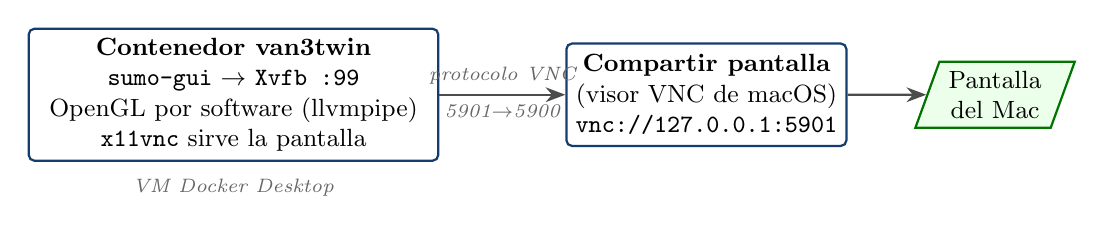
\begin{tikzpicture}[node distance=6mm and 10mm]
  \node[proceso, minimum width=52mm, minimum height=15mm] (cont)
    {\textbf{Contenedor van3twin}\\\texttt{sumo-gui} $\to$ \texttt{Xvfb :99}\\OpenGL por software (llvmpipe)\\\texttt{x11vnc} sirve la pantalla};
  \node[proceso, right=16mm of cont, minimum width=34mm, minimum height=13mm] (viewer)
    {\textbf{Compartir pantalla}\\(visor VNC de macOS)\\\texttt{vnc://127.0.0.1:5901}};
  \node[datos, right=10mm of viewer] (screen) {Pantalla\\del Mac};
  \node[etiq, below=1mm of cont] {VM Docker Desktop};
  \draw[flecha] (cont) -- node[etiq, above]{protocolo VNC}
                          node[etiq, below]{5901$\to$5900} (viewer);
  \draw[flecha] (viewer) -- (screen);
\end{tikzpicture}
\caption{Camino de la GUI por VNC: todo el pipeline gr\'afico (X + OpenGL)
corre dentro del contenedor y el Mac solo muestra el resultado.}
\label{fig:vncpath}
\end{figure}

Uso diario (dos pasos):

\begin{lstlisting}[language=bash, caption={En el Mac}]
open vnc://127.0.0.1:5901            # o Finder -> Cmd+K; dejar la ventana abierta
docker compose exec van3twin bash
\end{lstlisting}

\begin{lstlisting}[language=bash, caption={Dentro del contenedor}]
sumo-gui &        # prueba: la ventana de SUMO aparece en el visor VNC
./ns3 run "v2v-emergencyVehicleAlert-80211p"   # GUI activa por defecto
\end{lstlisting}

\begin{implicacion}
Al correr todo el pipeline gr\'afico dentro del contenedor, esta ruta no
depende de servidores X externos ni de GLX del Mac: es la opci\'on m\'as
robusta (y suele ser m\'as fluida que X11 sobre TCP), a costa de algo m\'as
de CPU. Xvfb y x11vnc son procesos: mueren al parar el contenedor y por eso
los relanza el \texttt{command} en cada arranque, sin pasos manuales. Todo
lo necesario (Xvfb, fluxbox, x11vnc, Mesa/llvmpipe, NetAnim) viene horneado
en la imagen: no se requiere ning\'un script auxiliar.
\end{implicacion}

\subsection{Alternativa: GUI v\'ia XQuartz (X11 en red)}

Si prefieres ventanas nativas de X11 en el escritorio del Mac (sin visor
VNC), existe la variante XQuartz. Requiere: instalar y configurar XQuartz
(\S\ref{sec:xquartzconf}), y activar en el compose las l\'ineas comentadas
(\texttt{DISPLAY: host.docker.internal:0} y
\texttt{LIBGL\_ALWAYS\_INDIRECT: "1"}, comentando a la vez
\texttt{DISPLAY: ":99"} y \texttt{LIBGL\_ALWAYS\_SOFTWARE}) seguido de
\texttt{docker compose up -d}.

\begin{figure}[h!]
\centering
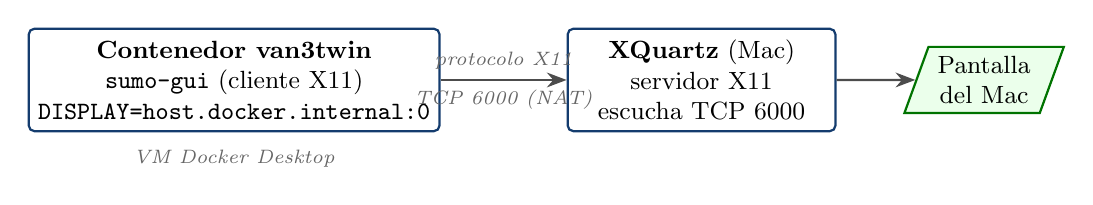
\begin{tikzpicture}[node distance=6mm and 10mm]
  \node[proceso, minimum width=44mm, minimum height=13mm] (cont)
    {\textbf{Contenedor van3twin}\\\texttt{sumo-gui} (cliente X11)\\\texttt{DISPLAY=host.docker.internal:0}};
  \node[proceso, right=16mm of cont, minimum width=34mm, minimum height=13mm] (xq)
    {\textbf{XQuartz} (Mac)\\servidor X11\\escucha TCP 6000};
  \node[datos, right=10mm of xq] (screen) {Pantalla\\del Mac};
  \node[etiq, below=1mm of cont] {VM Docker Desktop};
  \draw[flecha] (cont) -- node[etiq, above]{protocolo X11}
                          node[etiq, below]{TCP 6000 (NAT)} (xq);
  \draw[flecha] (xq) -- (screen);
\end{tikzpicture}
\caption{Camino de la GUI en la alternativa XQuartz: sumo-gui dibuja en la
pantalla del Mac a trav\'es del socket TCP de XQuartz.}
\label{fig:x11}
\end{figure}

\begin{lstlisting}[language=bash, caption={En el Mac}]
open -a XQuartz
/opt/X11/bin/xhost + 127.0.0.1
docker compose exec van3twin bash
\end{lstlisting}

\begin{advertencia}
Esta variante depende del GLX de XQuartz (\texttt{enable\_iglx}) y es la
fuente de los errores \texttt{GLXBadContext} / \texttt{No matching fbConfigs}
documentados en \S\ref{sec:trouble}. Si aparecen y no se resuelven, volver
al m\'etodo VNC por defecto (\S\ref{sec:vnc}), que no depende de XQuartz.
\end{advertencia}

\subsection{Visualizador web de veh\'iculos}

Algunos ejemplos integran el \texttt{vehicle-visualizer} (flag
\texttt{--vehicle-visualizer=true}); con el puerto 8080 ya publicado en el
compose, basta abrir \texttt{http://localhost:8080} en el navegador del Mac.
Requisitos y detalles en \S\ref{sec:vehviz}; para visualizar el
\emph{intercambio de mensajes} (Wireshark, NetAnim, PyViz), ver la
secci\'on~\ref{sec:visual}.

\subsection{Flujo de trabajo de desarrollo}

\begin{lstlisting}[language=bash]
# Editar código (dentro del contenedor, o con VS Code + extensión Dev Containers
# adjuntada al contenedor 'van3twin'):
nano src/automotive/examples/v2v-simple-cam-exchange-80211p.cc

# Recompilar (incremental, solo lo cambiado):
./ns3 build

# Exportar resultados al Mac:
cp mi-traza.csv ~/results/       # aparece en ~/van3twin-docker/results
\end{lstlisting}

\begin{nota}
Los cambios de c\'odigo y los builds incrementales quedan en la carpeta
\texttt{./VaN3Twin} del Mac: sobreviven a \texttt{docker compose down}, a
reinicios e incluso a borrar el contenedor y la imagen. Para versionar tu
trabajo, git normal desde el Mac (la carpeta es local); tambi\'en puedes
abrirla directamente en VS Code.
\end{nota}

\subsection{Ciclo de vida del contenedor}

\begin{lstlisting}[language=bash]
docker compose stop        # pausa (conserva el contenedor)
docker compose start       # reanuda
docker compose down        # elimina el contenedor (./VaN3Twin y ./results NO se tocan)
docker system df           # espacio usado por imágenes/volúmenes
\end{lstlisting}

\clearpage

% ============================================================================
\section{Visualizaci\'on de mensajes y de la simulaci\'on}
\label{sec:visual}
% ============================================================================

Cuatro herramientas complementarias, de m\'as a menos recomendada para
\emph{ver el intercambio de mensajes}: Wireshark (contenido real de cada
CAM/DENM), NetAnim (animaci\'on de paquetes entre nodos), PyViz
(vista interactiva en vivo) y el \texttt{vehicle-visualizer} de VaN3Twin
(mapa web de veh\'iculos; movilidad, no mensajes).

\subsection{Wireshark sobre los .pcap: el contenido de cada mensaje}
\label{sec:wireshark}

VaN3Twin transmite mensajes ETSI \emph{reales} (ASN.1 UPER sobre
BTP/GeoNetworking), y varios ejemplos ya generan capturas autom\'aticamente
mediante \texttt{EnablePcap()}: \texttt{v2v-simple-cam-exchange-80211p}
escribe \texttt{v2v-80211p-student-application-*.pcap} y
\texttt{v2v-emergencyVehicleAlert-80211p} escribe \texttt{v2v-EVA-*.pcap}
(un fichero por veh\'iculo, en \texttt{ns-3-dev/}). Wireshark disecciona la
pila completa: GeoNetworking (ethertype \texttt{0x8947}) $\to$ BTP $\to$
CAM/DENM con todos sus campos (posici\'on, velocidad, heading,
contenedores...).

Ejemplo completo:

\begin{lstlisting}[language=bash, caption={Dentro del contenedor}]
# ojo: este ejemplo no admite --sumo-gui (la GUI va fija); visor VNC abierto
./ns3 run "v2v-simple-cam-exchange-80211p --sim-time=30"
cp v2v-80211p-student-application-*.pcap ~/results/
\end{lstlisting}

\begin{lstlisting}[language=bash, caption={En el Mac}]
brew install --cask wireshark
open ~/van3twin-docker/results/v2v-80211p-student-application-0-0.pcap
\end{lstlisting}

En Wireshark: filtros de visualizaci\'on \'utiles: \texttt{gnw}
(GeoNetworking), \texttt{btpb} (BTP-B) e \texttt{its} (mensajes
CAM/DENM decodificados). El men\'u \emph{Statistics $\to$ Flow Graph}
genera un diagrama de secuencia del intercambio --- lo m\'as parecido a un
``visor de mensajes''.

\subsection{NetAnim: animaci\'on de paquetes entre nodos}
\label{sec:netanim}

NetAnim reproduce (offline) un XML generado por la simulaci\'on: nodos
movi\'endose y cada transmisi\'on como una flecha. El \'arbol ns-3 de
VaN3Twin ya incluye el m\'odulo \texttt{netanim}. \textbf{En la imagen
actual, el ejemplo \texttt{v2v-simple-cam-exchange-80211p} viene parcheado
de f\'abrica} (capa 6b del Dockerfile): genera
\texttt{v2v-cam-exchange-anim.xml} en cada ejecuci\'on sin tocar nada. Para
a\~nadir la animaci\'on a \emph{otro} ejemplo, estos son los tres cambios
(mostrados sobre
\texttt{src/automotive/examples/v2v-simple-cam-exchange-80211p.cc}):

\begin{lstlisting}[language=C++, caption={Cambio 1: junto al resto de \#include}]
#include "ns3/netanim-module.h"
\end{lstlisting}

\begin{lstlisting}[language=C++, caption={Cambio 2: justo ANTES de Simulator::Run() (l\'inea $\sim$362)}]
AnimationInterface anim ("v2v-cam-exchange-anim.xml");
anim.SetMaxPktsPerTraceFile (500000);
\end{lstlisting}

\begin{lstlisting}[caption={Cambio 3: enlazar el m\'odulo netanim en
src/automotive/examples/CMakeLists.txt (bloque del ejemplo, l\'inea
$\sim$125). Sin esto el enlace falla con \texttt{collect2: error: ld}.}]
build_lib_example(
        NAME v2v-simple-cam-exchange-80211p
        SOURCE_FILES v2v-simple-cam-exchange-80211p.cc
        LIBRARIES_TO_LINK
        ${libcarla}
        ${libautomotive}
        ${libwave}
        ${libtraci}
        ${libnetanim}
)
\end{lstlisting}

\begin{lstlisting}[language=bash, caption={Compilar el ejemplo y ejecutar}]
# dentro del contenedor
./ns3 build                      # recompila el ejemplo con la animacin
./ns3 run "v2v-simple-cam-exchange-80211p --sim-time=30"
# en el Mac (visor VNC abierto): abrir el visor, ya instalado en la imagen
docker compose exec van3twin NetAnim
# File > Open -> v2v-cam-exchange-anim.xml (generado en ns-3-dev/)
\end{lstlisting}

\begin{implicacion}
El visor NetAnim es una aplicaci\'on Qt5 que no existe en los repos de
Ubuntu: la imagen la compila durante el build y la deja instalada en
\texttt{/usr/local/bin/NetAnim}, lista para usar. Muestra
``paquetes'' gen\'ericos (qui\'en transmite a qui\'en y cu\'ando), no el
contenido ETSI: para el contenido, Wireshark (\S\ref{sec:wireshark}).
Con muchos veh\'iculos el XML crece r\'apido; \'usalo con simulaciones
cortas.
\end{implicacion}

\subsubsection*{C\'omo interpretar la ventana}

El lienzo de la pesta\~na \emph{Animator} es el plano cartesiano del mapa
SUMO, en \textbf{metros}. Cada punto rojo es un nodo ns-3 (un veh\'iculo),
numerado por orden de creaci\'on (0..N-1; el \texttt{veh1} de SUMO es el
nodo 0). Claves de lectura:

\begin{itemize}
  \item \textbf{Veh\'iculos ``aparcados'' en grupo} (t\'ipicamente en una
  esquina o sobre el origen): son nodos cuyo veh\'iculo a\'un no ha entrado
  en la simulaci\'on SUMO (o ya sali\'o); TraCI los mantiene fuera del mapa
  hasta su instante de inserci\'on. Es normal verlos incorporarse al
  recorrido a medida que avanza el reloj.
  \item \textbf{Flechas entre nodos} durante la reproducci\'on: cada
  transmisi\'on registrada. En 802.11p los CAM son \emph{broadcast}: un
  \'unico env\'io genera una flecha hacia cada receptor al alcance, por lo
  que la densidad de flechas es un proxy visual de la carga de canal.
  \item \textbf{Cadencia}: los CAM ETSI se emiten entre 10\,Hz y 1\,Hz
  seg\'un la din\'amica del veh\'iculo (reglas de generaci\'on ETSI); si un
  nodo ``parpadea'' m\'as, es que se mueve/gira m\'as.
\end{itemize}

\subsubsection*{Controles \'utiles}

\begin{itemize}
  \item \textbf{Barra superior}: play/pausa; \emph{Pause At} (detiene la
  reproducci\'on en un instante concreto); deslizador \emph{fast--slow}
  (intervalo de refresco de la animaci\'on: hacia \emph{slow} se ve cada
  transmisi\'on con calma); barra \emph{Sim time} para saltar a cualquier
  instante; rejilla (\texttt{\#} y \emph{Lines}); \emph{Node Size}
  (s\'ubelo a 2--4 para ver mejor los veh\'iculos); botones \emph{IP/MAC}
  (etiquetas de direcciones sobre cada nodo) y \emph{T} (trayectorias).
  \item \textbf{Barra izquierda}: lupas de zoom; bot\'on \emph{ID}
  (mostrar/ocultar n\'umeros de nodo); icono espiral (c\'irculos de
  transmisi\'on inal\'ambrica: dibuja el alcance de cada emisi\'on como
  onda, muy ilustrativo en V2X); icono de prohibido (oculta las flechas de
  paquetes si saturan la vista); \emph{(X,Y)} muestra las coordenadas del
  cursor para medir distancias sobre el mapa.
  \item \textbf{Pesta\~na Packets}: tabla de todas las tramas (instante,
  nodo origen $\to$ destino y metadatos 802.11/LLC); filtrable por nodo.
  Es el puente natural hacia Wireshark: aqu\'i ves \emph{cu\'ando y entre
  qui\'enes}, all\'i el \emph{contenido} ETSI.
  \item \textbf{Pesta\~na Stats}: contadores y propiedades por nodo.
\end{itemize}

Consejo operativo: mant\'en las simulaciones cortas
(\texttt{--sim-time=30}) --- el XML crece r\'apido con muchos CAMs --- y usa
\emph{Pause At} + zoom para analizar un evento concreto (p.\,ej.\ el
instante en que dos veh\'iculos entran en alcance mutuo).

\subsection{PyViz: vista interactiva en vivo}
\label{sec:pyviz}

PyViz (\texttt{--vis}) abre durante la simulaci\'on una ventana GTK con la
topolog\'ia en vivo: nodos, movimiento y \'ultimas transmisiones, con pausa
e inspecci\'on de nodos. Requiere los bindings Python de ns-3.

\begin{advertencia}
\textbf{Estado verificado en esta instalaci\'on (arm64, VaN3Twin master,
ago-2026): PyViz NO est\'a disponible.} Aunque el \texttt{configure} con
\texttt{--enable-python-bindings} pasa (v\'ia \texttt{pybindgen}), los
bindings \emph{pregenerados} del ns-3 original no compilan contra las
cabeceras que VaN3Twin parchea: fallan \texttt{propagation} y
\texttt{tap-bridge} (excluibles) y despu\'es m\'odulos esenciales del
n\'ucleo, que PyViz s\'i necesita. Es un problema de \emph{upstream}
(regenerar los bindings para el \'arbol parcheado), no de Docker ni de
Apple Silicon. Por ello la imagen compila por defecto con
\texttt{--disable-python}; si DriveX lo arreglara en el futuro, se puede
reintentar sin editar nada (hay fallback autom\'atico a sin-Python):

\begin{lstlisting}[language=bash]
docker compose build --build-arg NS3_PYTHON_FLAG=--enable-python-bindings
\end{lstlisting}

Las alternativas equivalentes, ya incluidas y funcionales, son
\textbf{NetAnim} (\S\ref{sec:netanim}) para la animaci\'on y
\textbf{Wireshark} (\S\ref{sec:wireshark}) para el contenido de los
mensajes.
\end{advertencia}

\subsection{PyViz vs.\ NetAnim: \textquestiondown cu\'al usar?}
\label{sec:pyviznetanim}

\begin{center}
\small
\begin{tabular}{@{}p{0.22\textwidth}p{0.34\textwidth}p{0.34\textwidth}@{}}
\toprule
\textbf{Criterio} & \textbf{PyViz} & \textbf{NetAnim} \\
\midrule
Momento & \textbf{En vivo}, durante la simulaci\'on (puede pausarla e
inspeccionar nodos). & \textbf{Offline}: reproduce despu\'es un XML grabado
por la simulaci\'on. \\
Puesta en marcha & \textbf{No disponible en este fork}: los bindings
pregenerados no compilan con los parches de VaN3Twin
(\S\ref{sec:pyviz}). & Visor ya instalado en la imagen; solo 2 l\'ineas
de c\'odigo en el ejemplo. \\
Interacci\'on & Alta: zoom, pausa, seguir un nodo, ver \'ultimas
transmisiones al vuelo. & Media: reproducir, rebobinar, cambiar velocidad,
estad\'isticas y tablas de paquetes. \\
Reproducibilidad & No deja traza: lo que ves se pierde al cerrar. & El XML
es un artefacto: se archiva, se comparte y se reproduce id\'entico (\'util
para papers y docencia). \\
Escalabilidad & Buena en vivo (no graba nada). & El XML crece r\'apido con
muchos veh\'iculos/CAMs: usarlo en simulaciones cortas. \\
Contenido mostrado & Topolog\'ia y transmisiones gen\'ericas (no decodifica
ETSI). & \'Idem: flechas de paquetes con metadatos b\'asicos. \\
\bottomrule
\end{tabular}
\end{center}

Regla pr\'actica: \textbf{NetAnim} si quieres una animaci\'on repetible y
barata de conseguir --- es la mejor relaci\'on esfuerzo/resultado en esta
instalaci\'on; \textbf{PyViz} queda descartado en esta
instalaci\'on mientras upstream no regenere los bindings
(\S\ref{sec:pyviz}). Y en ambos casos,
para el \emph{contenido} de los mensajes (campos del CAM/DENM), la
herramienta es Wireshark (\S\ref{sec:wireshark}): los animadores muestran
\emph{que} se transmite, no \emph{qu\'e} se transmite.

\subsection{vehicle-visualizer: mapa web de veh\'iculos}
\label{sec:vehviz}

El m\'odulo \texttt{src/vehicle-visualizer} muestra los veh\'iculos en vivo
sobre un mapa web (Leaflet). Requisitos, verificados en el c\'odigo del
m\'odulo:

\begin{itemize}
  \item \textbf{Node.js en el contenedor}: el modelo C++ comprueba
  \texttt{command -v node} y lanza \texttt{node server.js 8080 \&}. Ya viene
  en el Dockerfile actualizado; en contenedores previos:
  \texttt{sudo apt-get install -y nodejs}. (Las dependencias JS,
  \texttt{node\_modules}, vienen incluidas en el repo: no hace falta
  \texttt{npm install}.)
  \item \textbf{Puerto 8080 publicado}: ya est\'a en el compose
  (\texttt{8080:8080}); el socket UDP interno 48110 no necesita publicarse.
  \item \textbf{Activarlo por ejemplo}: los ejemplos que lo soportan exponen
  el flag \texttt{--vehicle-visualizer} (p.\,ej.\
  \texttt{v2v-emergencyVehicleAlert-80211p}, \texttt{v2i-*}).
  \item \textbf{Token de Mapbox: opcional.} Sin token, el mapa usa teselas
  est\'andar de OpenStreetMap (suficiente). Un token gratuito escrito en
  \texttt{src/vehicle-visualizer/js/mapbox\_token} habilita adem\'as las
  capas sat\'elite/h\'ibrida de Mapbox.
\end{itemize}

\begin{lstlisting}[language=bash]
# dentro del contenedor
./ns3 run "v2v-emergencyVehicleAlert-80211p --sumo-gui=false --vehicle-visualizer=true"
# en el Mac, con la simulacin corriendo:
open http://localhost:8080
\end{lstlisting}

\clearpage

% ============================================================================
\section{Sionna sin GPU: servidor nativo en el Mac}
\label{sec:sionna}
% ============================================================================

\subsection{An\'alisis: \textquestiondown se puede usar Sionna sin GPU NVIDIA?}

S\'i. El trazado de rayos de Sionna RT no lo hace TensorFlow sino
\textbf{Mitsuba~3 + Dr.Jit}, que tienen dos backends: CUDA (solo GPUs NVIDIA)
y \textbf{LLVM (CPU puro)}. Sin CUDA, Sionna cae autom\'aticamente al backend
LLVM. El propio script servidor del repo
(\texttt{src/sionna/sionna\_v1\_server\_script.py}) lo contempla con la
opci\'on \texttt{--gpu 0} (\emph{``set 0 to use CPU only''}).

La pregunta real es \emph{d\'onde} ejecutar el servidor. La integraci\'on es
desacoplada: ns-3 habla con el servidor Sionna por \textbf{UDP (puerto 8103)}
y la IP es configurable, as\'i que el servidor puede vivir fuera del
contenedor. Verificando los wheels publicados en PyPI para las versiones que
VaN3Twin soporta (v0.19 y v1.0):

\begin{center}
\small
\begin{tabular}{@{}llccc@{}}
\toprule
\textbf{Paquete} & \textbf{Versi\'on (fijada)} & \textbf{macOS arm64} &
\textbf{Linux aarch64} & \textbf{Linux x86\_64} \\
\midrule
\texttt{sionna}     & 1.0.2 (probada por DriveX) & \multicolumn{3}{c}{puro Python (depende de los de abajo)} \\
\texttt{sionna-rt}  & 1.0.2                      & \multicolumn{3}{c}{puro Python} \\
\texttt{mitsuba}    & 3.6.2 (fijada por sionna-rt) & \checkmark & \texttimes & \checkmark \\
\texttt{drjit}      & 1.0.3 (fijada por sionna-rt) & \checkmark & \texttimes & \checkmark \\
\texttt{tensorflow} & $\sim$2.19                 & \checkmark & \checkmark & \checkmark \\
\bottomrule
\end{tabular}
\end{center}

\begin{implicacion}
Consecuencias directas de la tabla:
\begin{itemize}
  \item \textbf{Dentro del contenedor arm64: no} (con las versiones
  soportadas): \texttt{mitsuba} 3.6.2 no publica wheels Linux aarch64;
  habr\'ia que compilar Mitsuba desde fuente. (Las versiones nuevas
  --- mitsuba 3.9 / sionna 2.x --- s\'i traen aarch64, pero DriveX no las ha
  probado.)
  \item \textbf{Contenedor amd64 + Rosetta: no}: TensorFlow x86\_64 requiere
  instrucciones AVX, que Rosetta~2 no emula (el proceso muere con
  \emph{illegal instruction}).
  \item \textbf{Nativo en macOS arm64: s\'i} --- todos los paquetes tienen
  wheels oficiales. Es la opci\'on recomendada sin GPU, y adem\'as usa los
  n\'ucleos del chip M directamente, sin el peaje de la VM.
\end{itemize}
\end{implicacion}

\begin{figure}[h!]
\centering
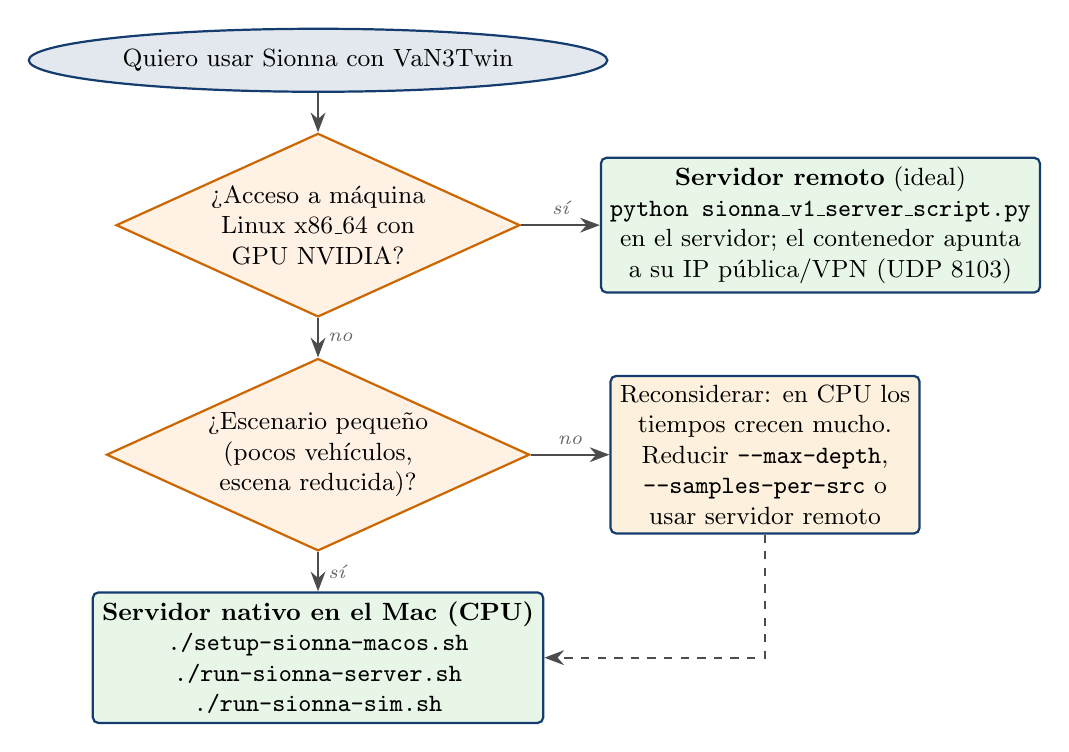
\begin{tikzpicture}[node distance=5mm]
  \node[inicio] (ini) {Quiero usar Sionna con VaN3Twin};
  \node[decision, below=of ini] (gpu) {\textquestiondown Acceso a m\'aquina\\Linux x86\_64 con\\GPU NVIDIA?};
  \node[proceso, right=10mm of gpu, fill=boximp] (remoto)
    {\textbf{Servidor remoto} (ideal)\\\texttt{python sionna\_v1\_server\_script.py}\\en el servidor; el contenedor apunta\\a su IP p\'ublica/VPN (UDP 8103)};
  \node[decision, below=of gpu] (tam) {\textquestiondown Escenario peque\~no\\(pocos veh\'iculos,\\escena reducida)?};
  \node[proceso, right=10mm of tam, fill=boxwarn] (warn)
    {Reconsiderar: en CPU los\\tiempos crecen mucho.\\Reducir \texttt{--max-depth},\\\texttt{--samples-per-src} o\\usar servidor remoto};
  \node[proceso, below=of tam, fill=boximp] (nativo)
    {\textbf{Servidor nativo en el Mac (CPU)}\\\texttt{./setup-sionna-macos.sh}\\\texttt{./run-sionna-server.sh}\\\texttt{./run-sionna-sim.sh}};
  \draw[flecha] (ini) -- (gpu);
  \draw[flecha] (gpu) -- node[etiq, above]{s\'i} (remoto);
  \draw[flecha] (gpu) -- node[etiq, right]{no} (tam);
  \draw[flecha] (tam) -- node[etiq, above]{no} (warn);
  \draw[flecha] (tam) -- node[etiq, right]{s\'i} (nativo);
  \draw[flecha, dashed] (warn) |- (nativo);
\end{tikzpicture}
\caption{Decisi\'on de despliegue del servidor Sionna cuando el Mac no tiene
GPU NVIDIA.}
\label{fig:sionnadecision}
\end{figure}

\subsection{Arquitectura de la soluci\'on nativa}

La figura~\ref{fig:sionnaarch} muestra las piezas y el flujo de datos: ns-3
publica las posiciones que recibe de SUMO y consulta al servidor los valores
de canal calculados por ray tracing.

\begin{figure}[h!]
\centering
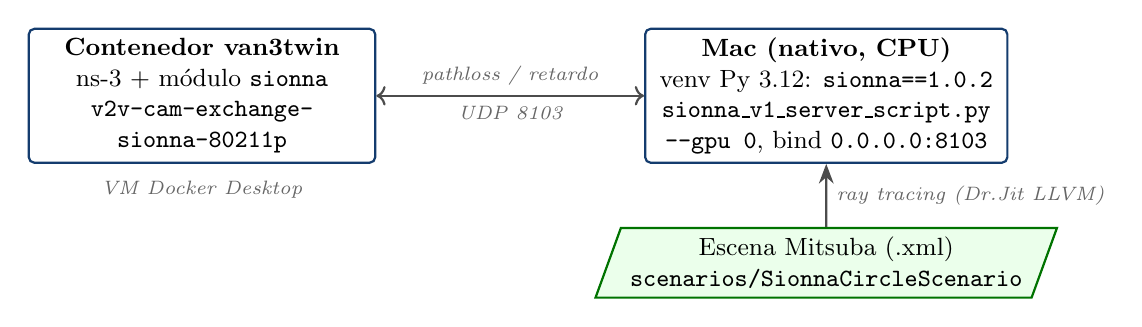
\begin{tikzpicture}[node distance=6mm and 12mm]
  \node[proceso, minimum width=44mm, minimum height=17mm] (cont)
    {\textbf{Contenedor van3twin}\\ns-3 + m\'odulo \texttt{sionna}\\\texttt{v2v-cam-exchange-}\\\texttt{sionna-80211p}};
  \node[proceso, right=34mm of cont, minimum width=46mm, minimum height=17mm] (srv)
    {\textbf{Mac (nativo, CPU)}\\venv Py 3.12: \texttt{sionna==1.0.2}\\\texttt{sionna\_v1\_server\_script.py}\\\texttt{--gpu 0}, bind \texttt{0.0.0.0:8103}};
  \node[datos, below=8mm of srv] (escena)
    {Escena Mitsuba (.xml)\\\texttt{scenarios/SionnaCircleScenario}};
  \node[etiq, below=1mm of cont] {VM Docker Desktop};
  \draw[flecha, <->] (cont) -- node[etiq, above]{pathloss / retardo}
                             node[etiq, below]{UDP 8103} (srv);
  \draw[flecha] (escena) -- node[etiq, right]{ray tracing (Dr.Jit LLVM)} (srv);
\end{tikzpicture}
\caption{Sionna nativo: ns-3 env\'ia posiciones de veh\'iculos (TraCI/SUMO) y
recibe p\'erdidas de propagaci\'on y retardos calculados por ray tracing en la
CPU del Mac. No se publica ning\'un puerto: el contenedor inicia la conexi\'on
saliente.}
\label{fig:sionnaarch}
\end{figure}

\subsection{Instalaci\'on (una sola vez)}

Con el contenedor ya construido (\S6), ejecutar desde la carpeta de trabajo:

\begin{lstlisting}[language=bash]
./setup-sionna-macos.sh
\end{lstlisting}

El script (Anexo~\ref{anexo:sionnasetup}) hace, en orden: instala
\texttt{python@3.12} y \texttt{llvm} con Homebrew si faltan; crea el venv
\texttt{\textasciitilde/van3twin-sionna} e instala \texttt{sionna==1.0.2} con
\texttt{tensorflow$\sim$=2.19}; copia \texttt{sionna\_v1\_server\_script.py} y
la carpeta \texttt{scenarios/} \emph{desde el contenedor} (\texttt{docker
compose cp}), garantizando que servidor y ns-3 usan exactamente la misma
versi\'on del protocolo; y verifica la importaci\'on de
\texttt{drjit}/\texttt{mitsuba}/\texttt{sionna.rt}.

\begin{implicacion}
Elecciones fijadas por compatibilidad de wheels: \textbf{Python 3.12} (techo
com\'un entre mitsuba 3.6.2 y TensorFlow 2.19 en arm64),
\textbf{TF $\sim$2.19} (sionna 1.0.2 exige \texttt{numpy<2.0} y excluye TF
2.16/2.17), y \textbf{LLVM de Homebrew} exportado v\'ia
\texttt{DRJIT\_LIBLLVM\_PATH} (Dr.Jit lo carga en tiempo de ejecuci\'on para
el backend CPU).
\end{implicacion}

\subsection{Ejecuci\'on}

\begin{lstlisting}[language=bash, caption={Terminal 1 (Mac): servidor Sionna en CPU}]
./run-sionna-server.sh            # bind 0.0.0.0:8103, --gpu 0
# opciones tiles en CPU: --verbose --max-depth 3 --samples-per-src 1000
\end{lstlisting}

\begin{lstlisting}[language=bash, caption={Terminal 2 (Mac): simulaci\'on en el contenedor}]
open vnc://127.0.0.1:5901         # este ejemplo abre sumo-gui SIEMPRE
./run-sionna-sim.sh
\end{lstlisting}

El script \texttt{run-sionna-sim.sh} (Anexo~\ref{anexo:sionnasim}) resuelve la
IP del host \emph{dentro} del contenedor y lanza:

\begin{lstlisting}[language=bash]
./ns3 run "v2v-cam-exchange-sionna-80211p --sionna=true --sionna-server-ip=$SIONNA_IP"
\end{lstlisting}

\begin{advertencia}
Tres detalles que ahorran horas de depuraci\'on:
\begin{itemize}
  \item El c\'odigo C++ de VaN3Twin usa \texttt{inet\_aton()}, que \textbf{no
  resuelve nombres DNS}: pasar \texttt{host.docker.internal} como
  \texttt{--sionna-server-ip} falla en silencio. Hay que pasar la IP num\'erica
  (el script la resuelve con \texttt{getent hosts}).
  \item El servidor debe arrancarse \textbf{sin} \texttt{--local-machine}:
  con ese flag har\'ia bind solo a \texttt{127.0.0.1} y el tr\'afico del
  contenedor (que llega por la VM) no lo alcanzar\'ia.
  \item El ejemplo \texttt{v2v-cam-exchange-sionna-80211p} tiene
  \texttt{SumoGUI} fijado a \texttt{true} en el c\'odigo (sin flag CLI):
  requiere la GUI activa --- abrir el visor VNC
  (\texttt{vnc://127.0.0.1:5901}, \S\ref{sec:vnc}) --- o editar esa
  l\'inea y recompilar.
\end{itemize}
La primera vez, el cortafuegos de macOS preguntar\'a si Python puede aceptar
conexiones entrantes: aceptar.
\end{advertencia}

\subsection{Expectativas de rendimiento en CPU}

El servidor mitiga el costo del ray tracing re-trazando solo cuando un
veh\'iculo se desplaza m\'as de 3\,m o gira m\'as de 90\textdegree{}
(\texttt{--position-threshold}, \texttt{--angle-threshold}) y cacheando
p\'erdidas y retardos. Aun as\'i, en CPU cada re-trazado toma segundos (frente
a milisegundos en GPU): es viable para escenas peque\~nas como
\texttt{SionnaCircleScenario} con pocos veh\'iculos, y se degrada r\'apido al
crecer la escena, \texttt{--max-depth} o el n\'umero de veh\'iculos. Para
campa\~nas de simulaci\'on grandes, usar la opci\'on de servidor remoto con
GPU (figura~\ref{fig:sionnadecision}).

\clearpage

% ============================================================================
\section{Soluci\'on de problemas}
\label{sec:trouble}
% ============================================================================

\begin{center}
\small
\begin{tabular}{@{}p{0.40\textwidth}p{0.52\textwidth}@{}}
\toprule
\textbf{S\'intoma} & \textbf{Causa y soluci\'on} \\
\midrule
\texttt{g++: internal compiler error: Killed (program cc1plus)} durante
\texttt{docker compose build} & OOM: la VM se qued\'o sin RAM. Subir memoria
en Docker Desktop (\S3.2) o bajar \texttt{cpus} y relanzar la build (contin\'ua
desde la capa cacheada). \\
\midrule
\texttt{sumo-gui: cannot connect to X server host.docker.internal:0}
\emph{(solo alternativa XQuartz)} &
XQuartz sin ``Allow connections from network clients'', o falta
\texttt{xhost + 127.0.0.1}, o XQuartz cerrado. Repetir
\S\ref{sec:xquartzconf} y reintentar --- o usar el m\'etodo VNC por defecto
(\S\ref{sec:vnc}). \\
\midrule
En el visor VNC las ventanas de SUMO salen sin bordes, inm\'oviles, sobre
fondo negro; o \texttt{sumo-gui} da \texttt{X Error: BadValue (major 150)} &
Xvfb arrancado sin gestor de ventanas y/o sin \texttt{+extension GLX}
(compose antiguo). Actualizar al compose actual (arranca
\texttt{fluxbox} y Xvfb con GLX) o dentro del contenedor:
\texttt{sudo apt-get install -y fluxbox; pkill x11vnc; pkill Xvfb} y recrear el
contenedor (\texttt{docker compose up -d}). \\
\midrule
\texttt{sumo-gui: cannot connect to X server :99} (m\'etodo VNC) & El
\texttt{Xvfb} interno no est\'a corriendo: contenedor creado con un compose
antiguo (sin el \texttt{command} que lo arranca) o imagen sin
\texttt{xvfb}. Reconstruir la imagen (\texttt{docker compose build}) y recrear el
contenedor (\texttt{docker compose up -d}). \\
\midrule
\texttt{X Error: code 161 ... GLXBadContext} repetido; la ventana de SUMO
abre pero el mapa no se dibuja \emph{(solo alternativa XQuartz)} & GLX
indirecto desactivado en XQuartz.
En el Mac: \texttt{defaults write org.xquartz.X11 enable\_iglx -bool true} y
reiniciar XQuartz.
Alternativa infalible (m\'as lenta), en el contenedor:
\texttt{LIBGL\_ALWAYS\_INDIRECT=0 LIBGL\_ALWAYS\_SOFTWARE=1 ./ns3 run ...} \\
\midrule
\texttt{libGL error: failed to load driver: swrast} (y sigue el
\texttt{GLXBadContext} aun con \texttt{LIBGL\_ALWAYS\_SOFTWARE=1}) & Dos
causas combinadas: (a) falta \texttt{libgl1-mesa-dri} en el contenedor
(\texttt{sudo apt-get install -y libgl1-mesa-dri mesa-utils}; ya en el
Dockerfile actualizado), y (b) \texttt{LIBGL\_ALWAYS\_INDIRECT=1} sigue
definido por el compose --- ponerlo \texttt{=0} puede no bastar: hay que
hacer \texttt{unset LIBGL\_ALWAYS\_INDIRECT}. Verificar con
\texttt{glxinfo -B} (debe reportar \texttt{llvmpipe}). Adem\'as, si XQuartz
no expone visuales GLX (iglx inactivo), el modo software contra XQuartz
tambi\'en falla: comprobar en el Mac \texttt{defaults read org.xquartz.X11
enable\_iglx} $\to$ 1 y cerrar XQuartz por completo antes de reabrir. \\
\midrule
Los errores GLX persisten con XQuartz haga lo que haga & Abandonar XQuartz y
usar la ruta VNC por defecto (\S\ref{sec:vnc}). No depende de GLX
del servidor de macOS y funciona siempre. \\
\midrule
\texttt{docker compose up} falla con \texttt{ports are not available ...
127.0.0.1:5900 ... address already in use} & El 5900 del Mac lo ocupa el
servicio \emph{Compartir pantalla}/Gesti\'on remota de macOS (o otro VNC).
El compose actualizado ya publica \texttt{127.0.0.1:5901:5900}; conectar a
\texttt{vnc://127.0.0.1:5901}. Diagn\'ostico: \texttt{sudo lsof -nP
-iTCP:5900 -sTCP:LISTEN}. \\
\midrule
\texttt{FXApp::openDisplay: unable to open display} seguido de
\texttt{Can not connect to sumo via traci ... Connection refused} & No es un
fallo de TraCI: SUMO muri\'o al no poder abrir la GUI (con VNC: Xvfb no
corriendo; con XQuartz: cerrado o sin \texttt{xhost}), y ns-3 no encontr\'o
el socket. Verificar la GUI (contenedor arriba y visor VNC abierto) y reintentar, o lanzar el ejemplo con
\texttt{--sumo-gui=false}. \\
\midrule
La GUI abre pero se cierra / errores \texttt{libGL} & \texttt{shm\_size}
insuficiente (subirlo a \texttt{2gb} en el compose) o, en la alternativa
XQuartz, falta \texttt{LIBGL\_ALWAYS\_INDIRECT=1}. \\
\midrule
\texttt{Please do NOT run this script as root} & Se ejecut\'o
\texttt{sandbox\_builder.sh} manualmente como root (p.\,ej.\ con
\texttt{docker exec -u root}). Usar siempre el usuario \texttt{vanet}. \\
\midrule
Tras \texttt{docker compose build}, el contenedor sigue ``viejo'' & La
carpeta \texttt{./VaN3Twin} (bind mount) tapa la imagen nueva. Renombrarla,
repoblarla desde la imagen nueva y recuperar del respaldo los cambios
propios. \\
\midrule
\texttt{no space left on device} & Disco virtual de Docker lleno. Aumentarlo
en Settings$\to$Resources y/o limpiar: \texttt{docker system prune -a}
(cuidado: borra im\'agenes no usadas). \\
\midrule
Build interrumpida a mitad de gRPC o ns-3 & Relanzar
\texttt{docker compose build}: el cach\'e de capas retoma desde la \'ultima
completada. Evitar que el Mac duerma: \texttt{caffeinate -i docker compose
build}. \\
\midrule
Al terminar la simulaci\'on: \texttt{recv: peer shutdown}, \texttt{Quitting
(on error)} y a veces \texttt{malloc\_consolidate()} & SUMO agot\'o su traza
antes de que ns-3 parase: el cliente TraCI encuentra el socket cerrado y el
proceso muere sucio \emph{despu\'es} de imprimir las estad\'isticas (los
resultados son v\'alidos). Cierre limpio: usar \texttt{--sim-time} menor que
la duraci\'on de la traza SUMO. \\
\midrule
\texttt{Fatal error} de TraCI al iniciar una simulaci\'on & Comprobar
\texttt{SUMO\_HOME} y que \texttt{sumo} responde
(\texttt{sumo --version}); ejecutar el ejemplo desde \texttt{ns-3-dev}
(el \texttt{working\_dir} del compose ya lo garantiza). \\
\midrule
La simulaci\'on Sionna se bloquea en ``Establishing remote connection'' o no
recibe respuestas & Servidor no arrancado, arrancado con
\texttt{--local-machine} (bind solo a 127.0.0.1), IP incorrecta (recordar:
\texttt{inet\_aton} no resuelve DNS) o cortafuegos de macOS bloqueando
Python. Ver \S\ref{sec:sionna}. \\
\midrule
\texttt{drjit}: error cargando LLVM en el Mac & Falta
\texttt{brew install llvm} o la variable \texttt{DRJIT\_LIBLLVM\_PATH}
(la exporta \texttt{run-sionna-server.sh}). \\
\midrule
Se necesita CARLA & Ver \S2.2: CARLA exige Linux x86\_64 + GPU
NVIDIA (usar un servidor remoto y apuntar la configuraci\'on
\texttt{CARLA-OpenCDA.conf} a \'el). Para Sionna sin GPU, ver
\S\ref{sec:sionna}. \\
\bottomrule
\end{tabular}
\end{center}

% ============================================================================
\section{Referencias}
% ============================================================================

\begin{itemize}
  \item Repositorio VaN3Twin: \url{https://github.com/DriveX-devs/VaN3Twin}
  \item Documentaci\'on oficial (ms-van3t):
        \url{https://ms-van3ts-documentation.readthedocs.io/en/master/}
  \item ns-3 fork 5G-LENA (CTTC): \url{https://gitlab.com/cttc-lena/ns-3-dev}
        (etiqueta \texttt{ns-3-dev-v2x-v0.2}) y m\'odulo \texttt{nr}
        (rama \texttt{nr-v2x-dev})
  \item SUMO: \url{https://sumo.dlr.de}
  \item Docker Desktop para Mac:
        \url{https://docs.docker.com/desktop/setup/install/mac-install/}
  \item XQuartz: \url{https://www.xquartz.org}
  \item Sionna --- instalaci\'on y requisitos (CPU/LLVM):
        \url{https://nvlabs.github.io/sionna/installation.html}
  \item Wheels de Mitsuba/Dr.Jit (verificaci\'on de arquitecturas):
        \url{https://pypi.org/project/mitsuba/},
        \url{https://pypi.org/project/drjit/}
\end{itemize}

\clearpage
\appendix

% ============================================================================
\section{setup-sionna-macos.sh (Sionna nativo, instalaci\'on)}
\label{anexo:sionnasetup}
% ============================================================================

\lstinputlisting[language=bash]{../setup-sionna-macos.sh}

\clearpage

% ============================================================================
\section{run-sionna-server.sh y run-sionna-sim.sh (Sionna nativo, ejecuci\'on)}
\label{anexo:sionnasim}
% ============================================================================

\lstinputlisting[language=bash]{../run-sionna-server.sh}

\lstinputlisting[language=bash]{../run-sionna-sim.sh}

\end{document}
